\documentclass{ltjsreport}
%\usepackage[dvipdfmx]{color}
\usepackage{geometry}
\usepackage{titlesec}
\usepackage{tocloft}
\usepackage{booktabs}
\usepackage{mathcomp}
\usepackage{array}
\usepackage{mathtools,amssymb}
\usepackage{siunitx}
\usepackage{multirow}
\usepackage{tabularx}
\usepackage{subcaption}
\usepackage{float}
\usepackage{listings,jvlisting}

\lstset{
	basicstyle={\ttfamily},
	identifierstyle={\small},
	commentstyle={\smallitshape},
	keywordstyle={\small\bfseries},
	ndkeywordstyle={\small},
	stringstyle={\small\ttfamily},
	frame={tb},
	breaklines=true,
	columns=[l]{fullflexible},
	%numbers=left,
	%xrightmargin=0zw,
	%xleftmargin=3zw,
	numberstyle={\scriptsize},
	stepnumber=1,
	numbersep=1zw,
	lineskip=-0.5ex,
	tabsize=2
}
\renewcommand{\lstlistingname}{ソースコード}

\geometry{
	left = 72truept,
	right = 72truept,
	top = 15truemm,
	bottom = 20truemm,
}

\titleformat{\chapter}% command
    [block]% shape
    {\bfseries\huge}% format
    {第 \thechapter 章}% label
    {0.5em}% sep
    {\leftline}% before-code
\titlespacing{\chapter}
    {0pt}% left
    {0pt}% before-sep
    {6pt}% after-sep

\renewcommand{\cfttoctitlefont}{\hfill\large\bfseries}
\renewcommand{\cftaftertoctitle}{\hfill\null}
\renewcommand{\cftbeforetoctitleskip}{0pt}
\renewcommand{\cftaftertoctitleskip}{0pt}

\renewcommand{\cftchapfont}{\normalsize}
% 章ページ番号のフォント
\renewcommand{\cftchappagefont}{\normalsize}
% 章番号の後に「:」を付ける
\renewcommand{\cftchapaftersnum}{:}
% 章見出しのインデント幅
\renewcommand{\cftchapnumwidth}{5em}
% 章見出しからページ番号までを点線でつなぐ
\renewcommand{\cftchapleader}{\cftdotfill{\cftchapdotsep}}
% 点線の点間隔の調整
\renewcommand{\cftchapdotsep}{\cftdotsep}
% 章見出しの上にある余白を調整
\setlength{\cftbeforechapskip}{0pt}

\makeatletter
  \def\Hline{
  \noalign{\ifnum0=`}\fi\hrule \@height 3.\arrayrulewidth \futurelet
  \reserved@a\@xhline}
\makeatother

\begin{document}
%タイトルページ
\newgeometry{
	%余白調整
	top=70truemm,
	bottom = 10truemm,
}
\begin{titlepage}
\begin{center}
\huge 令和5年度\\
\vspace{30pt}
\huge 卒業研究報告書\\
\vspace{50pt}
\HUGE\textgt{仮想筋電義手の開発に関する研究}\\
\vspace{250pt}
\huge 指導教員\hspace{10pt}戸崎 哲也\\
\huge 報告者\hspace{28pt}河合 将暉\\
\vspace{50pt}
\huge 神戸市立工業高等専門学校\\
\huge 電子工学科
\end{center}
\end{titlepage}
\restoregeometry
\clearpage
%タイトルぺージここまで

%ページ番号をローマ数字で表示
\pagenumbering{roman}
%論文要旨
\begin{center}
\LARGE (論文要旨)
\end{center}
上肢切断者が筋電義手を装着し,日常生活で扱えるようになるには相応の訓練が必要とされる.
この筋電義手の訓練を代替するものとして,仮想筋電義手シミュレータが先行研究によって開発
されてきた.本研究では,先行研究で一般的に使用されていた配布されている仮想筋電義手3Dモ
デルとは異なる3Dスキャナ``EinScan HX''を用いた仮想筋電義手3Dモデルを使用することにより
筋電義手装着訓練の訓練効果に影響があるかを検討した.また,入力インターフェースにFirstVRを
採用することによる訓練効果への影響を検討するために,シミュレータのプロトタイプを提案した.
手法として,3Dスキャナで実際の左腕から3Dモデルを取得し,ノイズ成分をBlenderのスムージング
機能を用いて3Dモデル表面の平滑化を行った.その3Dモデルにボーン配置を行い,Unityにインポート
することで物体保持アニメーションを作製し,筋電義手の動作と似た動作をするようなシステム構成にした.
ここで,キーボード・マウスを入力インターフェースとしたPC版のシミュレータでは実際の上肢切断者
が操作できないという課題点を``FirstVR''を導入することで解決した.FirstVRは腕に巻くだけで
3軸ジャイロセンサや加速度センサにより腕の位置をトラッキングすることが可能であり,加えて
筋変位センサによるジェスチャ認識機能も備わっている.これにより,仮想筋電義手シミュレータ
が実際の上肢切断者でも扱えるようになった上に,筋変位によるジェスチャ認識のしきい値を
実際の筋電義手に近づけることにより訓練効果の向上を見込めると考えた.

本研究では前段階として,FirstVRのジェスチャ認識率,最適サンプル数の調査と,健常者を対象にした6段階リッカート尺度
を用いた定性評価アンケート調査を行い,入力インターフェースをキーボード・マウスとしたシステムと
FirstVRのシステムとを比較した.まず,FirstVRのジェスチャ認識率は実験協力者各個人による分散が大きく,
最高値は100%,最低値は50%と大幅に差ができてしまっている.おそらくジェスチャ認識率が70%以下の場合では
複合的な要因が考えられ,装着位置や各個人の筋肉量の違いによって差ができていると考察した.
このため,sample数を比較する際に個人差が含まれないように80%未満のデータを除外すると,
どのsample数においても96.6 ± 3.34%のジェスチャ認識率が結果として得られた.
これより,ジェスチャ認識率では最適sample数を導くことはできなかった.
これを踏まえて,評価指標を独自に導入することにより,各筋変位センサの測定値ごとに比較し,実験協力者
による分散がもっとも少なく,データの学習量が小さいものを最適sample数とした.
この評価指標により,sample数7が最適であるとして,シミュレータを構成した.
次に,定性評価アンケート調査ではFirstVRのシステムがより没入感が高いという結果が得られた.しかし,
操作性や入力遅延といった点では優位性がみられることはなく,さらにFirstVRの装着位置・ジェスチャ学習のプロセスなどの
条件を加えて改善することが求められる.
\clearpage
%論文要旨ここまで

%目次を節まで表示に設定
\setcounter{tocdepth}{2}
%目次を表示
\tableofcontents

\clearpage
%ページ番号をアラビア数字に設定
\pagenumbering{arabic}


\chapter{はじめに}
	\section{研究背景}
		上肢切断者が筋電義手を装着する際,自在に扱うことができるように
		訓練を行う必要がある.VRを用いた筋電義手トレーニングの効果に
		ついては先行研究\cite{ref:1}\cite{ref:2}で検討されており,筋電
		義手操作の幻肢痛緩和やに効果があると立証されている.これらの研
		究では仮想筋電義手の3Dモデルについては長方形のオブジェクトや,
		腕を模して製作された3Dモデルを用いることが一般的であった.
		また,近年では``カグラ''\cite{ref:3}という医療機器は上肢機能障害者
		のリハビリテーションのために運用されるなどVRトレーニングシステムは
		義手装具者以外にも需要が高まっている.本研究は2023年度,神戸高専
		Digital Faburication Labに新規導入されたハンディ3Dスキャナ``Ein Scan HX''\cite{ref:4}の活用方法の一例として後続の研究に
		利用していただきたい.

		本論文の構成として第2章,第3章で3Dモデルの製作やUnity・FirstVRについて
		解説を行う.そして,第4章に研究手法を提示し,第5章に研究結果を示す.

	\section{関連研究}
		FirstVRを用いた関連研究としては足にFirstVRを装着することで足の筋変位による
		足の接地状態の検出を行う研究\cite{ref:6}が行われている.この研究では
		図\refeq{fig:RR-FVRcalibration}の歩行状態を7段階に分割した姿勢をFirstVRにそれぞれ学習させ,加えてジャイロセ
		ンサを用いてどの姿勢が足の接地状態(立脚期)の検出に最適なのかを調査されている.
		\begin{figure}[H]
		\centering
		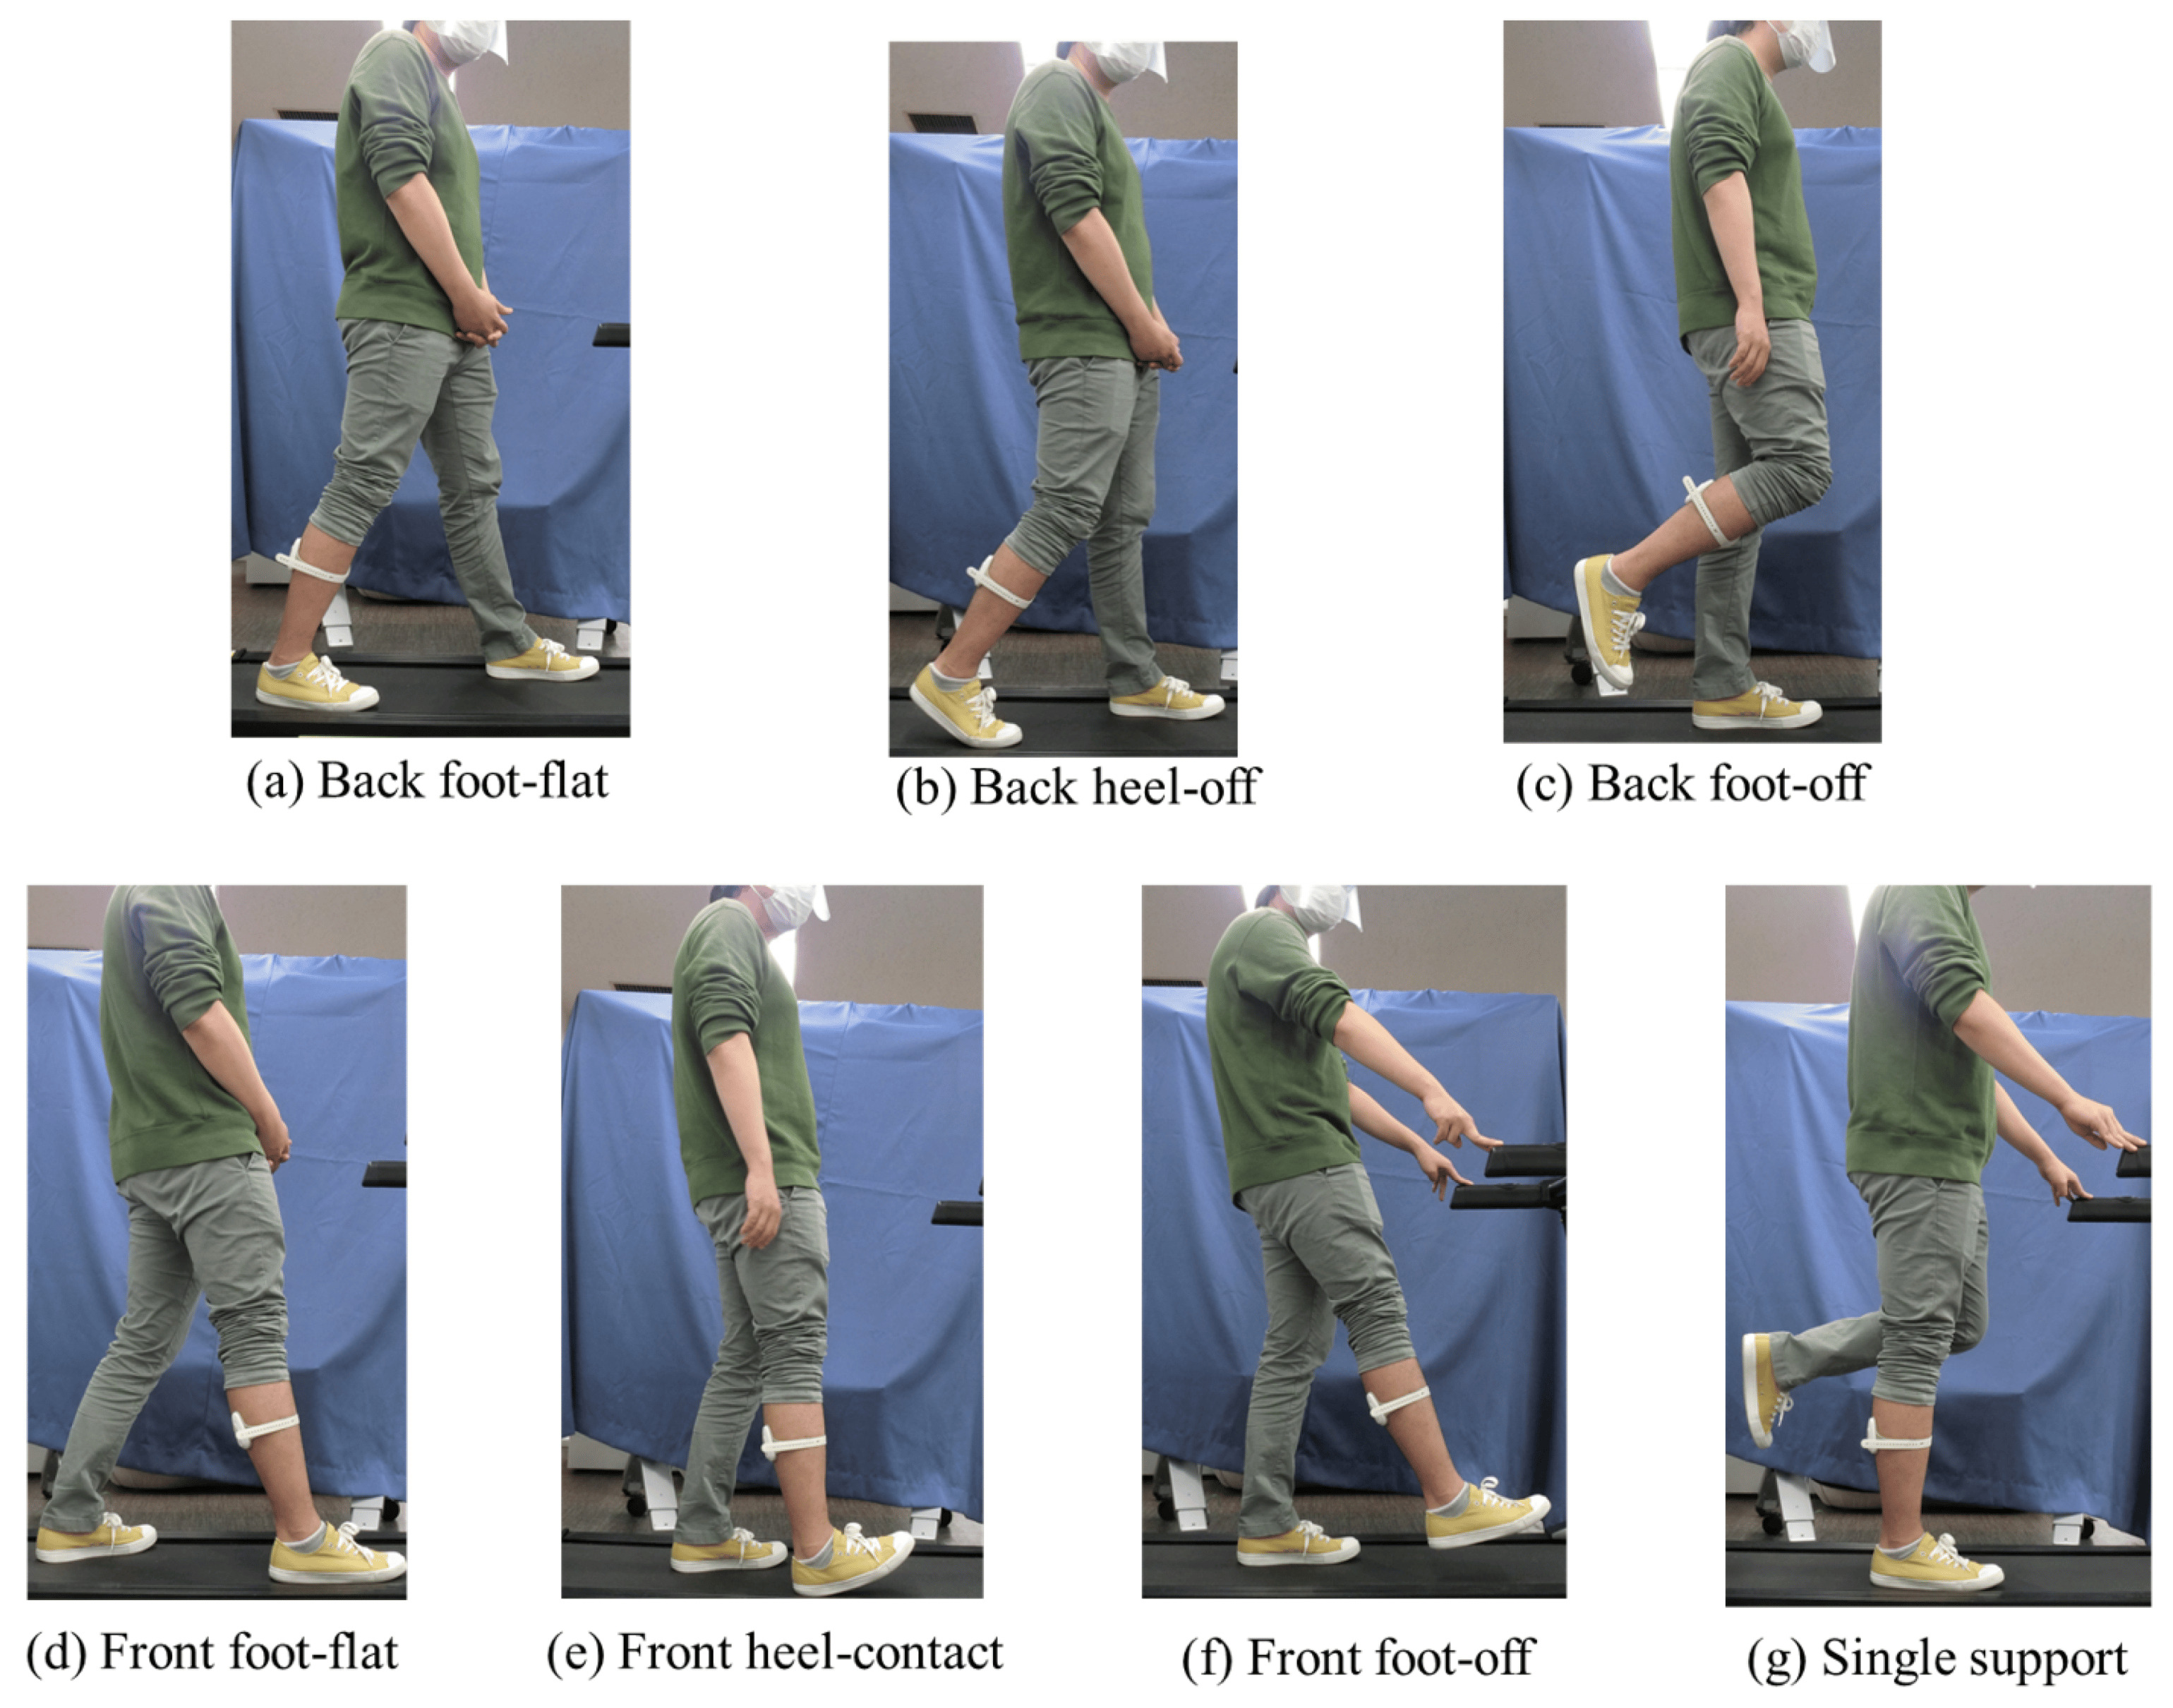
\includegraphics[width = 8cm]{../figs/sensors-21-01081-g004.jpg}
		\rightline{文献\cite{ref:6}より引用}
		\caption{歩行位相検出アルゴリズムのキャリブレーション姿勢}
		\label{fig:RR-FVRcalibration}
		\end{figure}

		文献\cite{ref:6}によると,足の浮遊状態(遊脚期)の検出には体軸よりも足が後ろになっている状態が検出精度が高くなる
		傾向にあるということが報告されており,その姿勢状態を学習させて実験協力者10名(男性6名,女性4名)
		にトレッドミルを用いて歩行データを計測されていた.
\clearpage
		文献\cite{ref:6}より引用した男女別の
		遊脚期(Swing phase)と立脚期(Stance phase)の陽性率を図\refeq{fig:RR-malefemale}に示す.

		\begin{figure}[H]
		\centering
		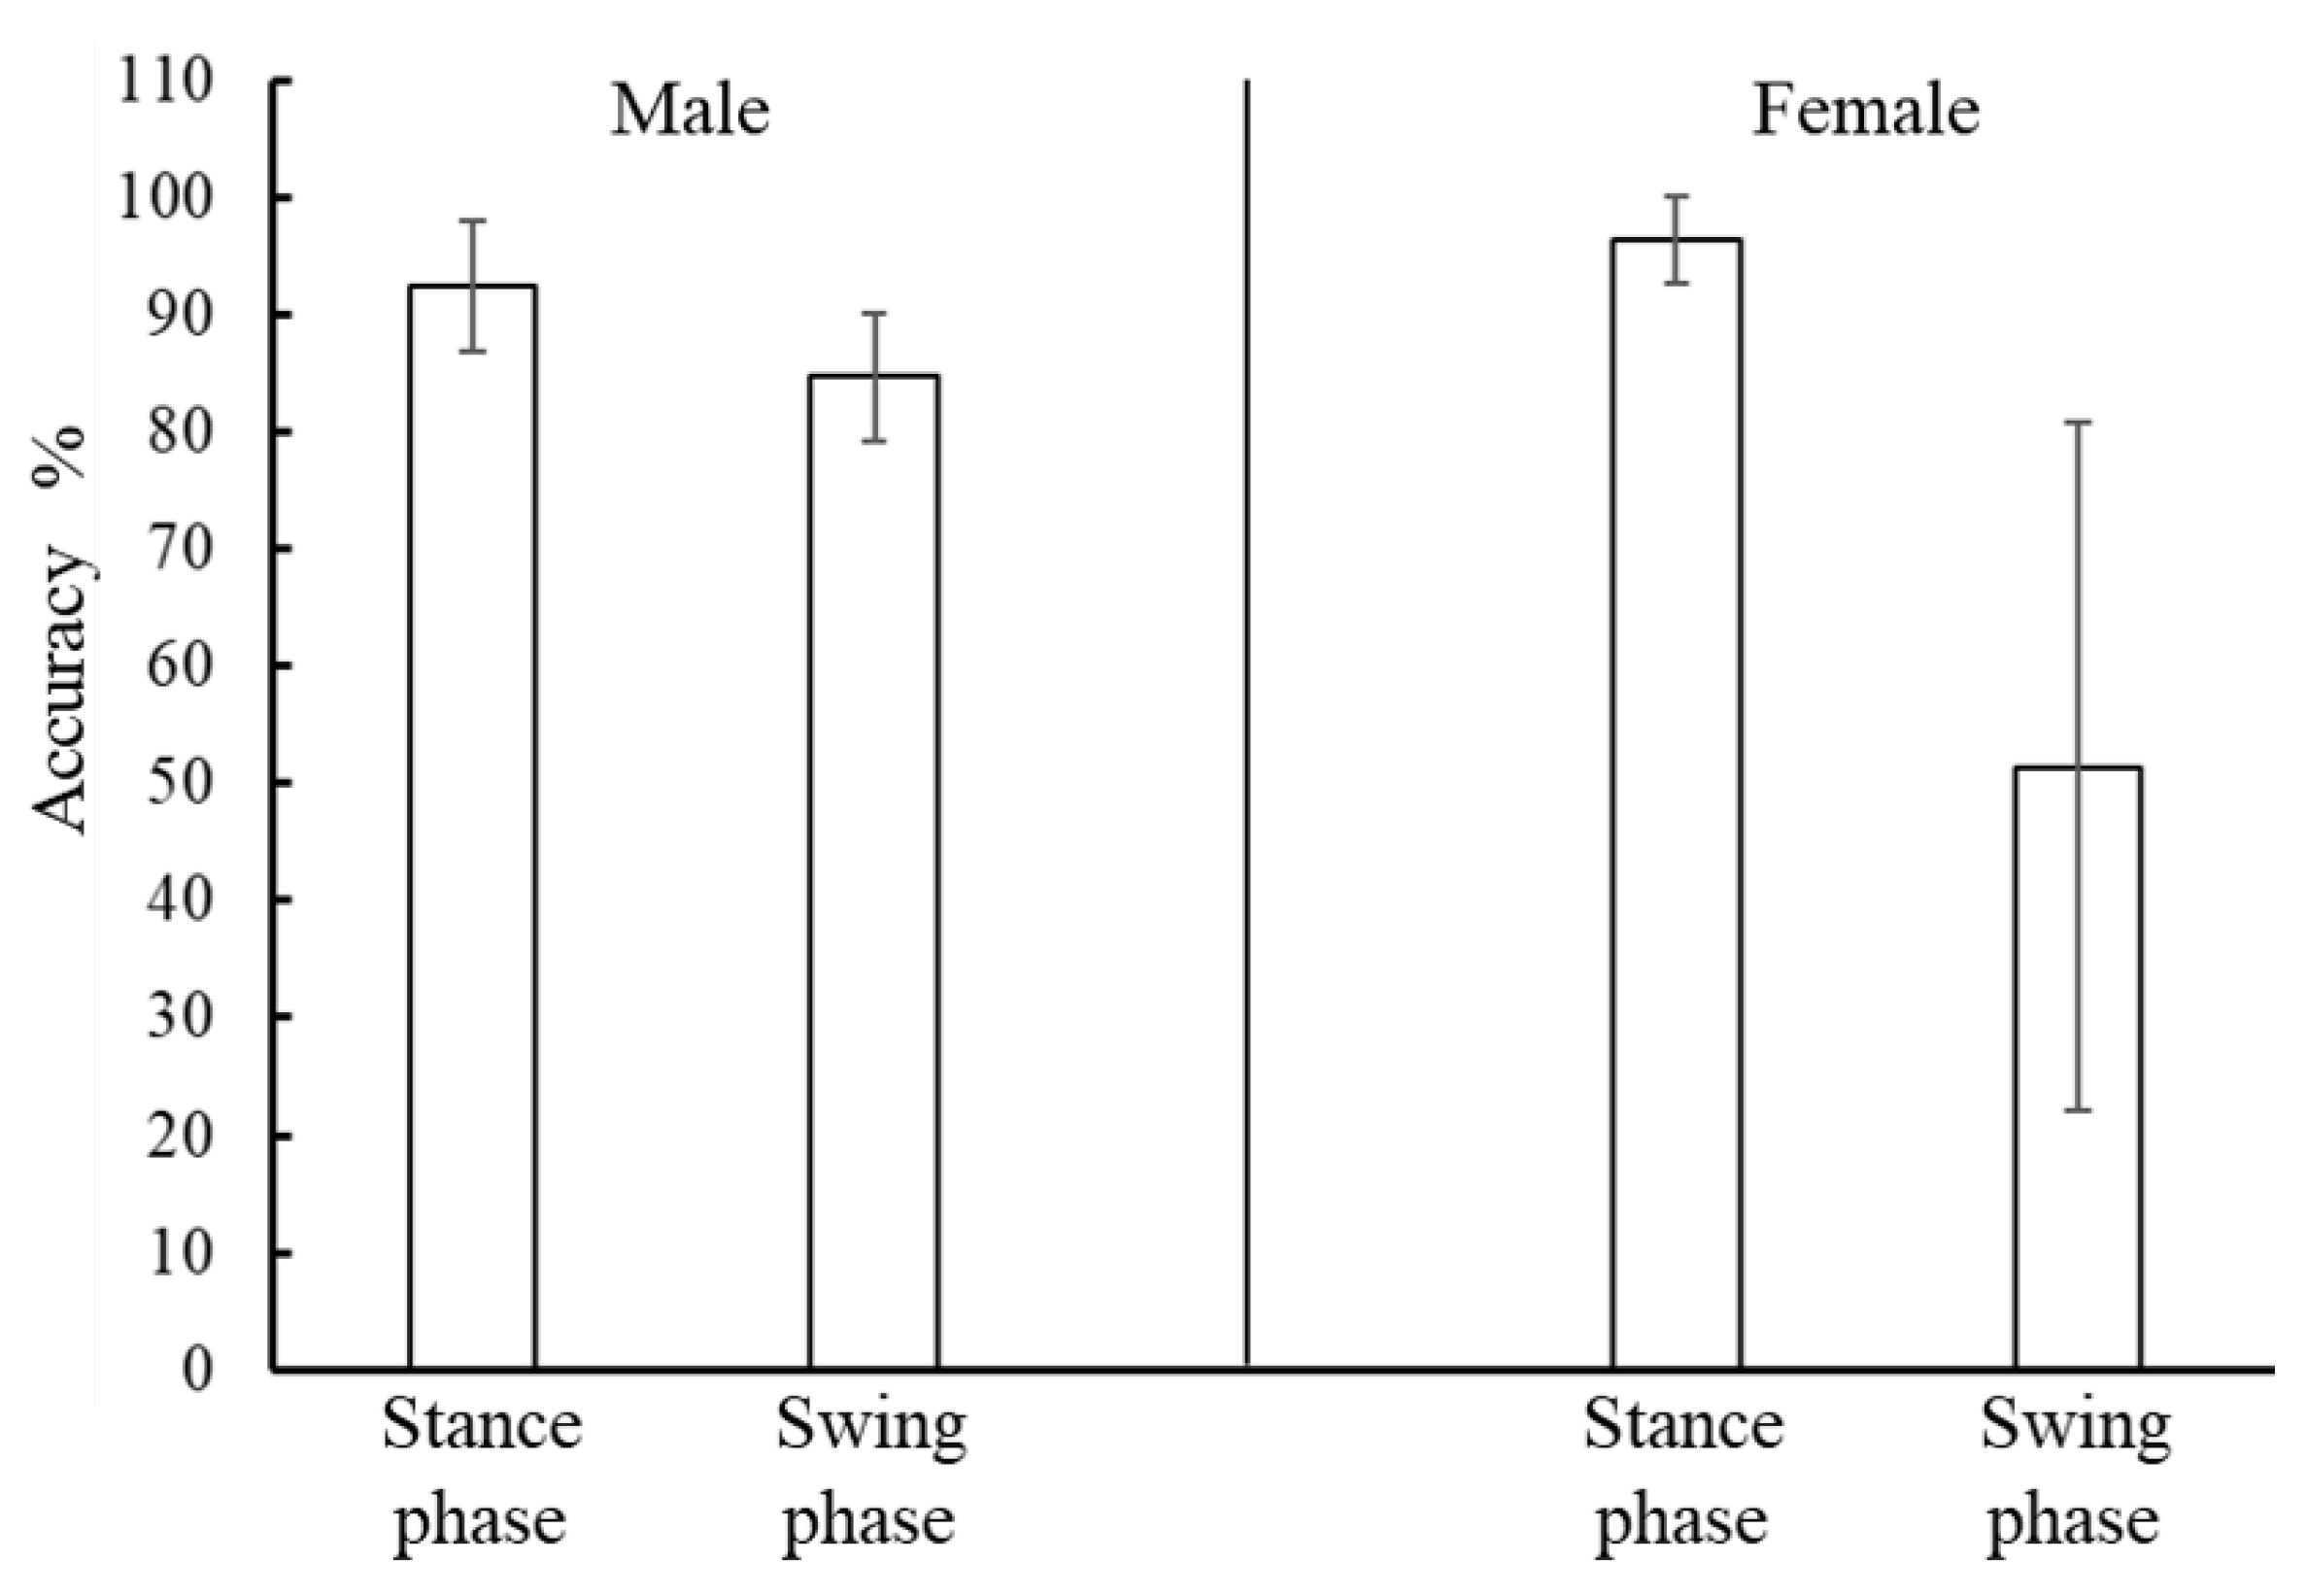
\includegraphics[width = 8cm]{../figs/sensors-21-01081-g010.jpg}
		\rightline{文献\cite{ref:6}より引用}
		\caption{男性(左)と女性(右)の立脚期と遊脚期の陽性率\\}
		\label{fig:RR-malefemale}
		\end{figure}

		図\refeq{fig:RR-malefemale}の結果より,立脚期の検出精度中央値は90%であり,
		歩行位相検出システムとして十分な結果を得られている.しかし,この方式では
		女性の遊脚期の検出精度が低いことから個人の筋肉量に検出精度が依存している
		といった課題がこの研究によって報告されている.

		\section{研究目的}
		本研究では,仮想筋電義手モデルのリアリティによる訓練効果や幻
		肢痛緩和効果に着目し3Dスキャナで取り込んだ仮想筋電義手3Dモデル
		(VH:Virtual Hand)を用いたVRトレーニングシステムを構成し,VHの
		見た目によって訓練効果に変化があるかを評価することを目的とする.
		加えて,このトレーニングシステムのインタフェースに``FirstVR''\cite{ref:5}
		を用いることで,実際の筋電義手や高価な筋電センサ使用することな
		く,安価で訓練が行えると考えたため,FirstVRによる訓練効果の影響を
		調べるために前段階として性能評価や定性評価を行い,入力インターフェースに
		よる没入感や操作性などの違いを調査することにした.


\chapter{3Dモデルの製作}
	本章では,3Dモデル製作に使用した``Ein Scan HX''と``Blender''について解説する.
	また,それぞれの役割と機能についても説明を加える.

	\section{EinScan HX}
		EinScan HXは株式会社サンステラが提供するハンディ3Dスキャナである.
		主な使用用途としては,工業製品などの比較的大きな物をスキャンし,
		リバースエンジニアリングや測定などに用いられている.
		図\refeq{fig:EinScan}にEinScanの外観を示す.

		\begin{figure}[H]
		\centering
		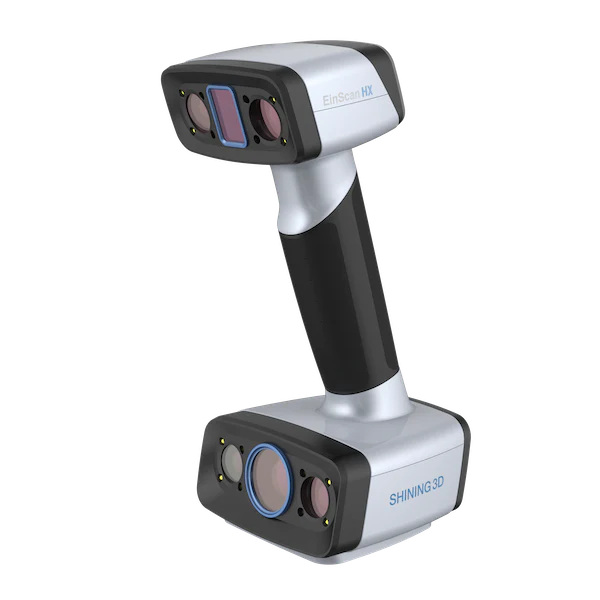
\includegraphics[width = 5cm]{../figs/EinScan.png}
		\caption{EinScan HX}
		\label{fig:EinScan}
		\end{figure}

		\subsection{製品仕様}
			文献\cite{ref:4}から引用したEinScanの製品仕様を図\refeq{fig:EinScan}に示す.
			\begin{table}[H]
			\begin{center}
			\caption{EinScan HXの製品仕様}
			\label{tab:EinScan}
			\begin{tabular}{c|cc} \Hline
				スキャン形式&Rapidスキャン&レーザースキャン\\ \hline
				スキャン精度&0.05\,mm&0.04\,mm\\
				ポイント間隔&0.25~3.00\,mm&0.05~3.00\,mm\\
				被写体長3D精度&±0.1\,mm&±0.06\,mm\\
				シングルスキャン精度&420 × 440\,mm&380 × 400\,mm\\
				光源&ブルーLED&ブルーレーザー7本\\
				被写体深度&200-700\,mm&350-610\,mm\\
				対象物との距離&470\,mm&470\,mm\\
				テクスチャスキャン&あり&なし\\
				安全性&クラス対象外&クラス1\\ \hline
				データ出力形式&\multicolumn{2}{c}{STL,OBJ,PLY,ASC,3MF,P3}\\
				本体サイズ&\multicolumn{2}{c}{108×110×237\,mm}\\
				本体重量&\multicolumn{2}{c}{710\,g}\\ \Hline
			\end{tabular}
			\rightline{文献\cite{ref:4}から引用}
			\end{center}
			\end{table}
			ここで,被写体長3D精度というのはスキャン時に取得するポイントの
			最大累積誤差を示したもので,測定する点数が増える場合や
			取得点の距離が大きい場合に誤差が累積し,大きくなっていく.

	\section{Blender}
		Blenderとは,オープンソースの完全無料統合型3DCG・2D・映像編集ソフトウェア
		である.本研究では``EinScan HX''によって出力した.obj形式の3Dモデルを
		編集する目的で使用した.次項からは本研究で用いたBlenderの機能について解説する.
		\subsection{スムージング}
			スムージング機能とは,\cite{ref:7}によると3Dオブジェクト等の点群データにおいて,ノイズを削減するために
			近傍データを用いて平均化処理を行い,データ点列をスムーズになるようにすることである.
			Blenderでは,この処理をペイントツールのようにオブジェクトをなぞるだけでその軌跡に従うように平均化処理が行われている.
			スムージング処理のイメージ画像を図\refeq{fig:smoothingEX}に示す.
			\begin{figure}[H]
			\centering
			\begin{minipage}{0.25\columnwidth}
			\centering
			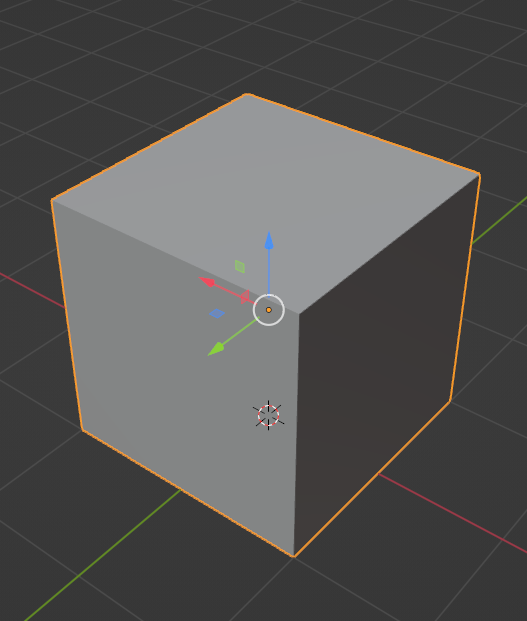
\includegraphics[width = \columnwidth]{../figs/SmoothingBeforCube.png}
			\end{minipage}
			\hspace{0.04\columnwidth}
			\begin{minipage}{0.25\columnwidth}
			\centering
			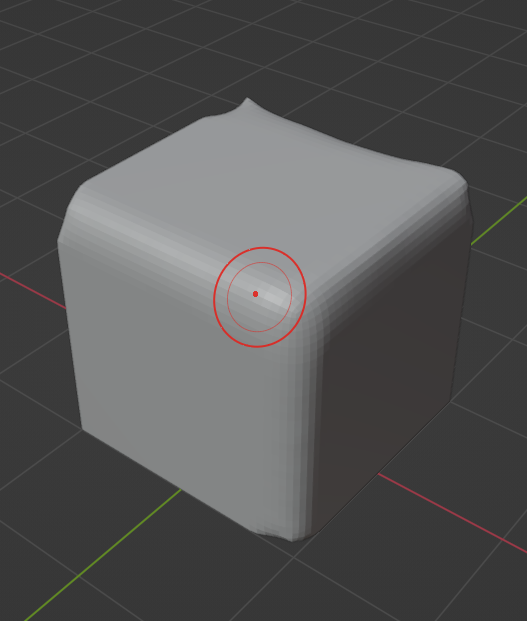
\includegraphics[width = \columnwidth]{../figs/SmoothingAfterCube.png}
			\end{minipage}
			\caption{頂点数35000点の立方体オブジェクトのスムージング処理比較}
			\label{fig:smoothingEX}
			\end{figure}
		\subsection{ボーン構成}
			ボーンは,3Dオブジェクトを変形させる際に頂点の移動を制御する支柱の役割を果たす機能である.
			Unityにインポートした後に物体保持のアニメーションを作成する際,VHの変形を制御するために用いている.
			ボーンによるメッシュ変形の様子を図\refeq{fig:bonecontrol}に示す.
			\begin{figure}[H]
			\centering
			\begin{minipage}{0.3\columnwidth}
			\centering
			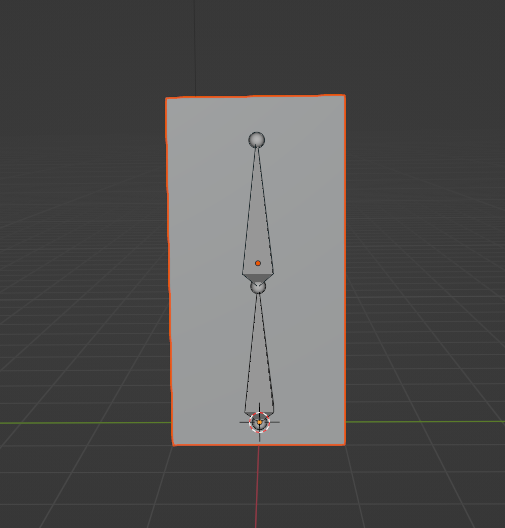
\includegraphics[width = \columnwidth]{../figs/bone1.png}
			\end{minipage}
			\hspace{0.04\columnwidth}
			\begin{minipage}{0.3\columnwidth}
			\centering
			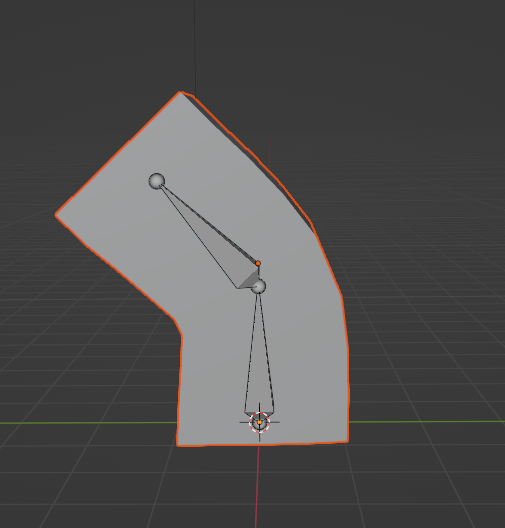
\includegraphics[width = \columnwidth]{../figs/bonecheck.png}
			\end{minipage}
			\caption{ボーンによるメッシュ変形制御}
			\label{fig:bonecontrol}
			\end{figure}


	\section{Unity}
		Unityは,Unity Technologies社が提供するゲーム制作を中心とした統合開発環境のことで,主にスマートフォン向けゲームの制作に用いられている.
		特徴としては,他社製の開発環境よりも比較的簡単にゲームの制作をすることが可能で,プログラムを必須としない点に強みをもつ.
		本研究ではVRトレーニングシステムを構築する上で利用した機能について解説を加える.
		\subsection{シェーダー}
			本研究では,UnityにインポートしたVHの見た目をよりリアルにするため,標準搭載のシェーダーではなく,``Reflex Shader 2.2''というシェーダーを
			用いて表示した.このシェーダーは主にVRChatの3Dモデル表示に用いられ,標準のシェーダーと比較して鏡面光が抑制され,モデルのコントラストが強調されていることがわかる.
			\begin{figure}[H]
			\centering
			\begin{minipage}{0.4\columnwidth}
			\centering
			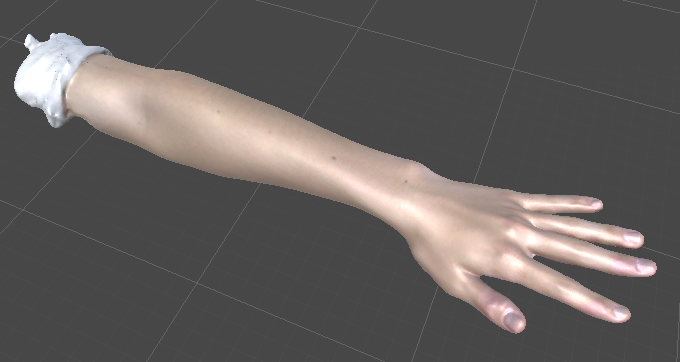
\includegraphics[width = \columnwidth]{../figs/NomalShader.png}
			\subcaption{Unity標準シェーダー}
			\end{minipage}
			\hspace{0.04\columnwidth}
			\begin{minipage}{0.4\columnwidth}
			\centering
			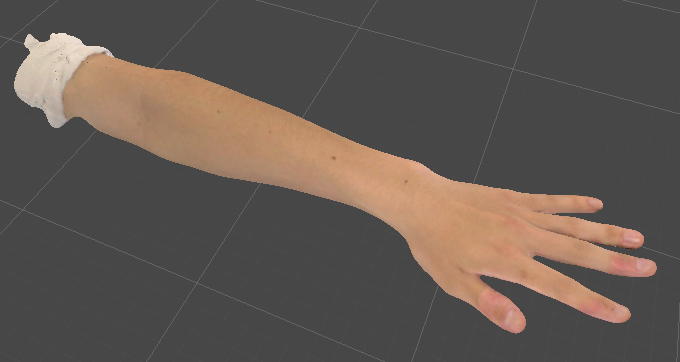
\includegraphics[width = \columnwidth]{../figs/ReflexShader.png}
			\subcaption{Reflex Shader}
			\end{minipage}
			\caption{シェーダーによる3Dモデルの違い}
			\label{fig:Shader}
			\end{figure}

		\subsection{衝突判定}
			本研究では衝突判定にUnityに標準搭載されているColliderコンポーネントとRaycastコンポーネントを用いた
			衝突判定を行った.次項にそれぞれの衝突判定の違いについて解説する.
			\subsubsection{Collider}
				Colliderコンポーネントにはオブジェクトの被衝突領域を設定する役割があり,
				異なる2つのオブジェクトに付加されたColliderの領域が重なることで衝突フラグを立てる.
				本研究ではPC版シミュレータにこの方式の衝突判定を用いている.

		\subsubsection{Raycast}
			Raycastコンポーネントはオブジェクトの中心から任意方向・任意長さに直線を引き,その直線と
			Colliderコンポーネントを持つオブジェクトの被衝突領域が重なると衝突フラグを立てる.
			本研究ではiOS版シミュレータにこの方式の衝突判定を用いている.
			\begin{figure}[H]
			\centering
			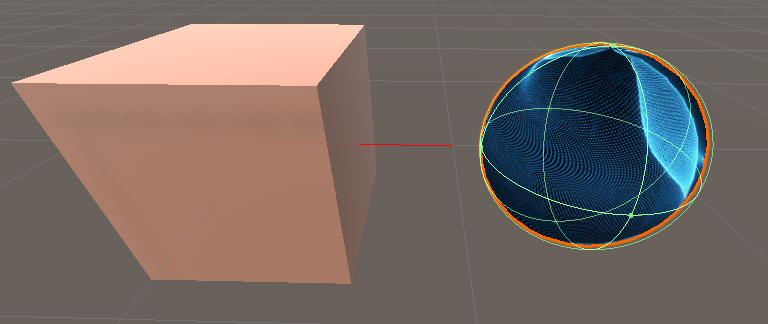
\includegraphics[width = 12cm]{../figs/raycast.png}
			\caption{Raycastのイメージ図}
			\label{fig:Raycast}
			\end{figure}

			図\refeq{fig:Raycast}のように左側の立方体オブジェクトの中心から射出されている赤い直線がRayである.
			この直線と右側の球体オブジェクトを囲う黄緑の領域がColliderコンポーネントの被衝突領域となっている.
			なお,図\refeq{fig:Raycast}のRayやColliderは表示されないようになっている.

		\subsection{アニメーション}
			オブジェクト保持状態を表現するためにVHにオブジェクトごとの保持アニメーションを作製した.
			Unityにおけるアニメーションは各オブジェクトの動きを記録し,再生フラグが立った場合にアニメーションが再生されるようになっている.
			また,アニメーションを作製する際,初期状態とアニメーションした後のオブジェクトの位置を記録することで
			自動的にその移動が補完されるようになっている.図\refeq{fig:animationclip}にアニメーションクリップ機能の画面を示す.

			\begin{figure}[H]
			\centering
			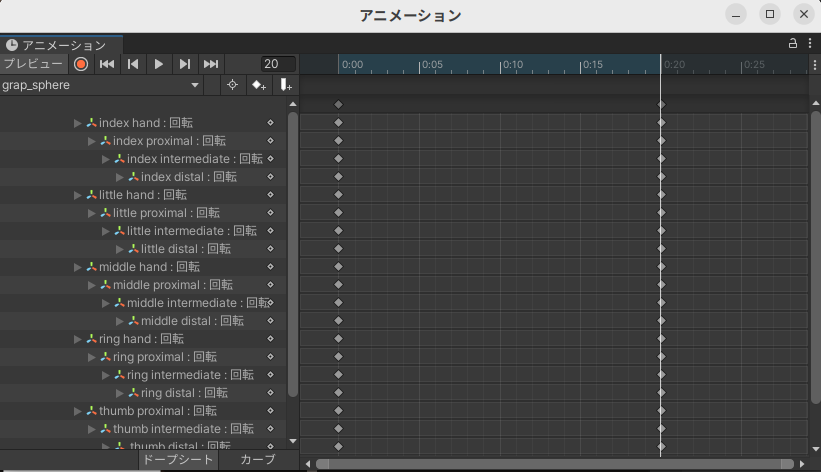
\includegraphics[width = 12cm]{../figs/animationclip.png}
			\caption{アニメーションクリップ機能}
			\label{fig:animationclip}
			\end{figure}

			複数のアニメーションの状態遷移を制御する役割としてアニメーター機能がUnityに備わっている.
			図\refeq{fig:animater}の動作ではシーンの実行直後に緑色ブロックのEntryからオレンジブロックのGrapSphereに遷移し,
			アニメーションが実行され,赤色ブロックのEndに遷移する.アニメーター機能では,遷移条件を付加することも可能である.

			\begin{figure}[H]
			\centering
			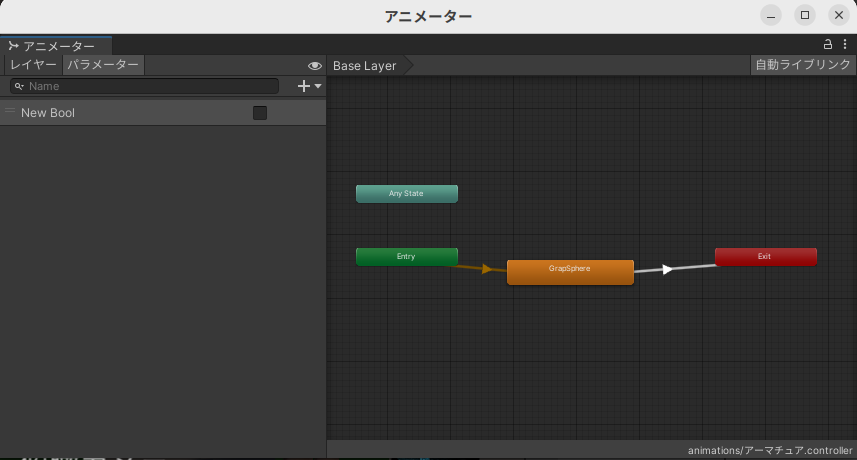
\includegraphics[width = 12cm]{../figs/animaterexample.png}
			\caption{アニメーター機能}
			\label{fig:animater}
			\end{figure}

		\subsection{ビルド}
			本項ではUnityで構成したシミュレータのビルド方法について解説する.
			以下にビルドの手順を示す.
			\begin{enumerate}
				\item Unityエディタ上のツールバーから"File"を選択
				\item ``Build Settings''の項目を選択すると,別ウィンドウにBuild Settingsが開かれる
				\item 追加したいシーンファイルをUnityエディタ上で開いておき,Build Settingsのウィンドウから"Add Open Scenes"を選択
				\item Build Settings ウィンドウの左にあるPlatformから実行したいOSを選択し,ウィンドウ右下の"Switch Platform"を選択
				\item Build Settings ウィンドウ右下の"build"を選択してビルド開始
			\end{enumerate}
			以上の手順でUnityで作成したシーンのビルドが完了する.
			Windows,LinuxなどのOSではビルドしたフォルダに実行ファイルが作成されているため,
			そのファイルからシミュレータを実行することができる.また,AndroiOSに関しても,作成した実行ファイルを
			AndroidOSに転送し,ファイル解凍することで実行できる.

			\begin{figure}[H]
			\centering
			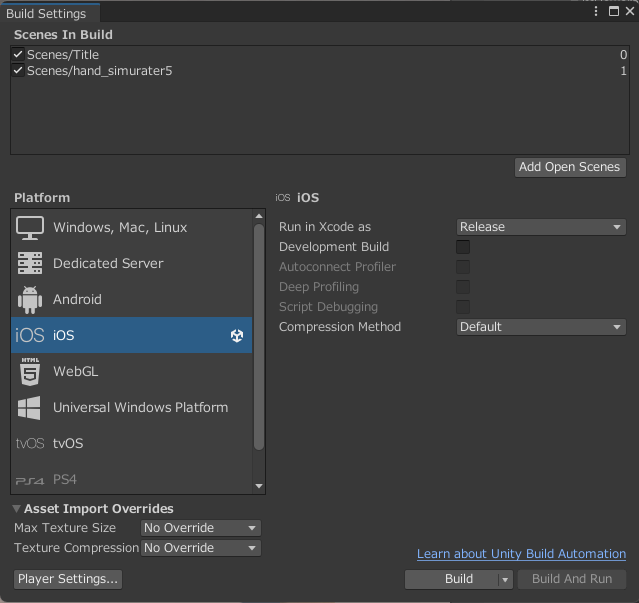
\includegraphics[width = 10cm]{../figs/BuildSettings.png}
			\caption{BuildSettings画面}
			\label{fig:BuildSettings}
			\end{figure}

			iOSに関してはビルド・実行方法が異なるため,以下に解説する.
			\subsubsection{iOSのビルド方法}
				本項では,iOS用アプリの実行手順を以下に示す.
				\begin{enumerate}
					\item ビルドされたフォルダをMacOSに転送
					\item MacOSでビルドされたフォルダを開き,フォルダ内の``Unity-iPhone.xcodeproj''をXcodeで開く
					\item iOS端末を接続し,端末の設定から端末をデバッグモードにする
					\item Xcodeウィンドウ上部のAny iOS Device を選択し,接続した端末を選択
					\item Signing&Capabilitiesを選択し,Teamの欄にApple IDを入力
					\item 本シミュレータではBluetoothを用いるため,infoを選択し,Keyの一覧に``Privacy - Bluetooth Peripheral Usage Description''を追加
						し,Valueを``Uses BLE to communicate with devices.''にする
					\item iPhoneにアプリがインストールされたら,端末の『設定』から『プライバシーとセキュリティ』を開き『Bluetooth』を選択
					\item インストールしたアプリにBluetoothの権限を許可する
					\item アプリ一覧からインストールしたアプリを実行する
				\end{enumerate}
				以上の手順でiOS用のシミュレータをビルドして実行できる.
				この手順で一番重要なのが,6の手順でこれがなければアプリを実行してもMade by Unityのポップがでた
				直後に動かなくなってしまう.これらのエラーはXcode上でログが残されているため,発生しているエラーを
				解消すれば実行することができる.大抵の場合,端末側の権限付与ができておらずアプリが実行できないエラーが多発するため
				よく確認をすること.
	\section{FirstVR}
		FirstVRはH2L株式会社\cite{ref:5}によって開発・製造されている筋変位センサを用いたウェアラブルデバイスである.
		この製品は現状iOSとAndroidのみ対応しており,アプリケーション開発をする際はH2Lから公開されている``FirstVR sdk''というUnity開発用APIが公開されている
		\subsection{デバイス構成}
				FirstVRの外観を図\refeq{fig:FirstVR}に示す。
				\begin{figure}[H]
				\centering
				\begin{minipage}{0.75\columnwidth}
				\centering
				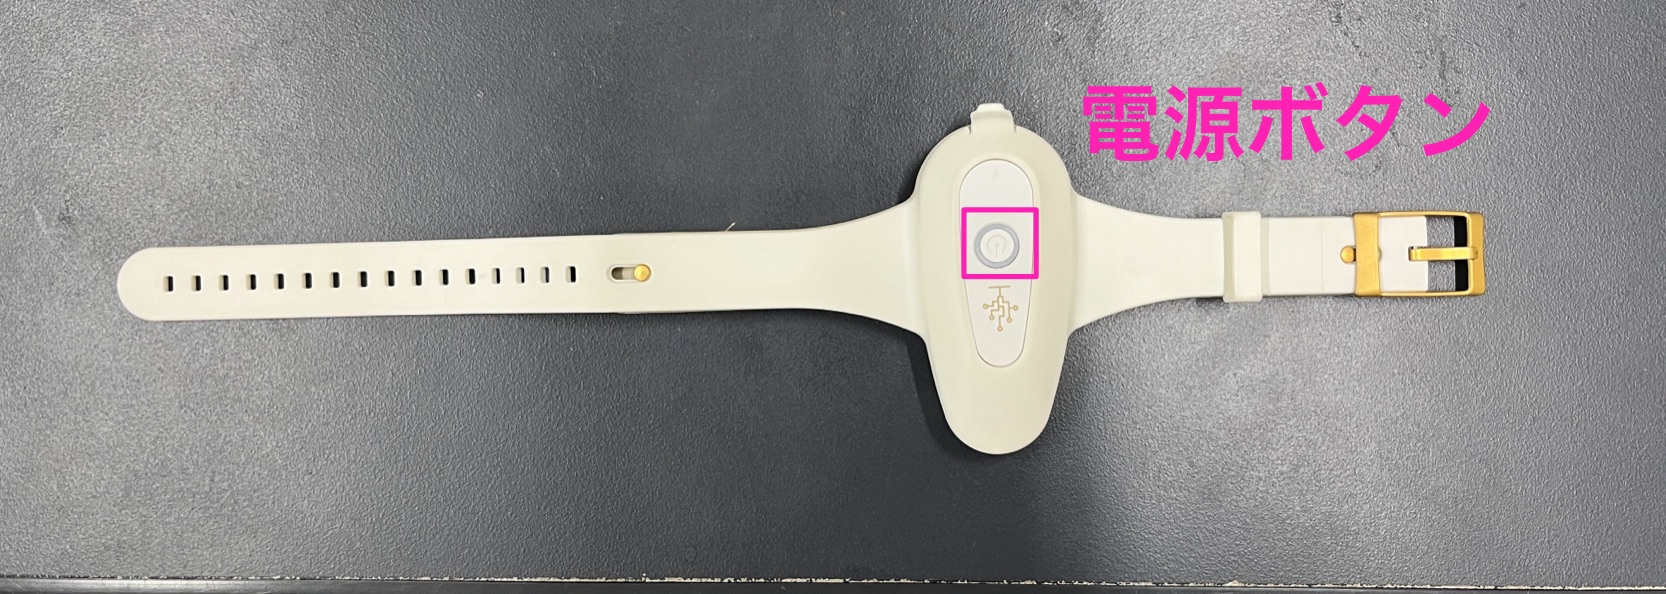
\includegraphics[width = \columnwidth]{../figs/IMG_0337.JPG}
				\subcaption{表面画像}
				\end{minipage}
				\hspace{0.04\columnwidth}
				\begin{minipage}{0.75\columnwidth}
				\centering
				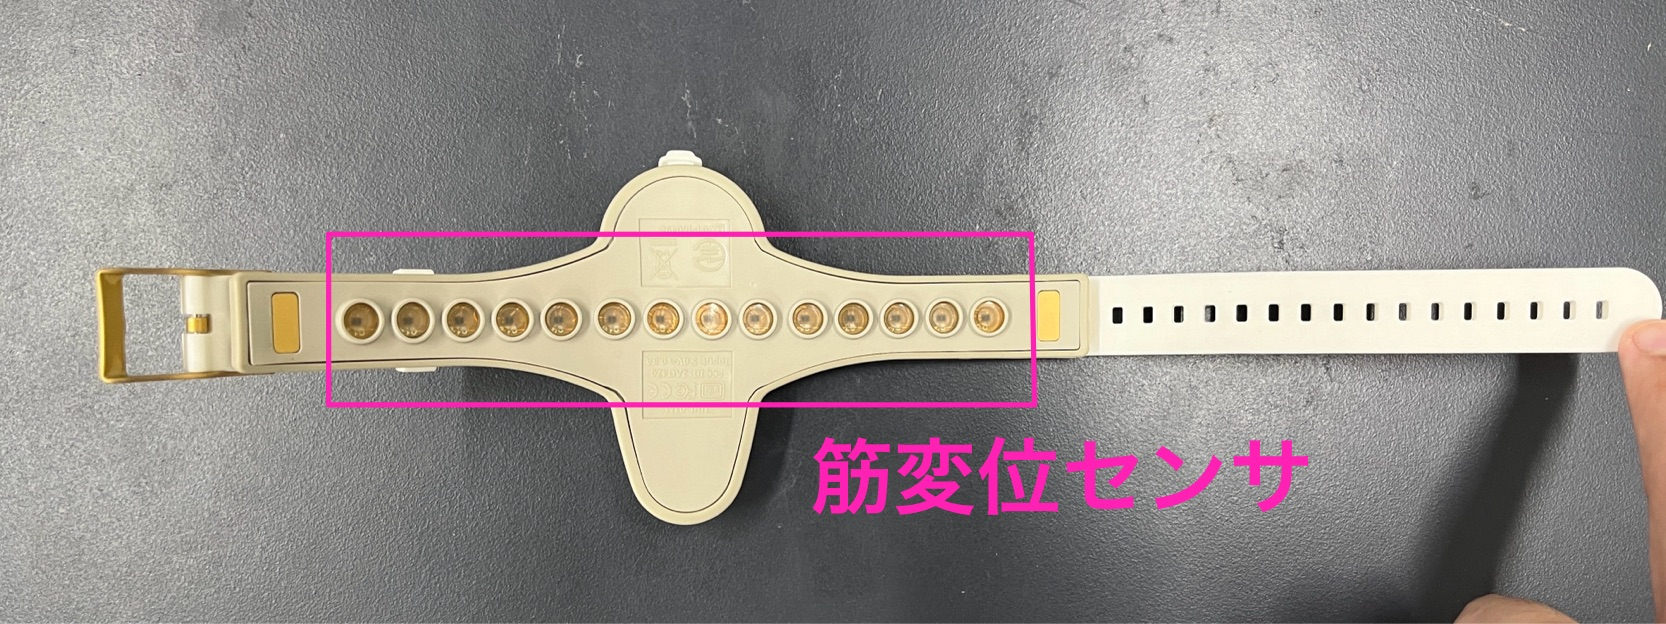
\includegraphics[width = \columnwidth]{../figs/IMG_0336.JPG}
				\subcaption{裏面画像}
				\end{minipage}
				\caption{FirstVR}
				\label{fig:FirstVR}
				\end{figure}

\vspace{-5pt}
			裏面には筋変位センサが14チャンネル配置されており,ここから装着した筋肉の変位を
			測定している.筋変位センサは近赤外線を射出し肌表面に反射させることで距離を測定し,
			その値を筋変位センサの測定値として出力している.

		\subsection{トラッキング}
			FirtVRには3軸ジャイロセンサと加速度センサが搭載されており,Unityで作製したアプリ上で測定値を
			確認することができる.本研究ではこのジャイロセンサを用いて,腕のピッチ,ヨー,ロールの3軸の
			回転をシミュレータに反映させている.
		\subsection{ジェスチャ認識}
			FirstVRのジェスチャ認識方法は,ジェスチャ状態と非ジェスチャ状態における筋変位センサの
			各チャンネルごとの値をサンプリングし,機械学習させることでジェスチャ状態のセンサ値を
			しきい値としてジェスチャ認識を行っている.

\chapter{研究手順}
	\section{使用器具}
		本研究での使用器具を表\refeq{tab:usedev}に示す.
	\begin{table}[H]
	\begin{center}
	\caption{本研究における使用器具}
	\label{tab:usedev}
	\begin{tabular}{clllll} \Hline
	No&\multicolumn{1}{l}{機器名}&\multicolumn{1}{l}{型番}&\multicolumn{1}{l}{シリアルNo}&\multicolumn{1}{l}{備考}\\ \hline
	1&EinScan HX&&&\\
	2&FirstVR&UHL-01&&\\
	3&スマートフォン1&iphone SE2&&iOS16.7.2\\
	4&スマートフォン2&iphone 13&&iOS17.2.1\\
	5&スマートフォン3&HUAWEI Nova Lite2&&AndroidOS 9\\
	6&PC-1&&&Ubuntu22.04\\
	7&PC-2&Mac mini2&&MacOS\\
	\Hline
	\end{tabular}
	\end{center}
	\end{table}
	本研究で使用したソフトウェアを表\refeq{tab:usesoft}に示す.
	\begin{table}[H]
	\begin{center}
	\caption{使用ソフトウェア}
	\label{tab:usesoft}
	\begin{tabular}{clllll} \Hline
	No&\multicolumn{1}{l}{ソフトウェア名}&\multicolumn{1}{l}{バージョン}&\multicolumn{1}{l}{使用OS}&\multicolumn{1}{l}{備考}\\ \hline
	1&Blender&3.0.1&Ubuntu&\\
	2&Unity&2022.3.11f1&Ubuntu&\\
	3&Xcode&15.0.1&MacOS&\\
	\Hline
	\end{tabular}
	\end{center}
	\end{table}
	\section{VHの3Dモデル取り込み}
		ハンディ3DスキャナであるEinScan HXを用いて左腕をスキャンする.
		本研究では,VHにテクスチャを貼って用いることを前提としているため,
		スキャン形式をRapidスキャンモードで,3Dモデルの精度を高めるために
		頂点数を50万点で出力し,出力形式としてテクスチャがメッシュに割当
		されているobj形式を選択する.

	\section{VHのスムージング処理・ボーン配置}
		obj形式で取り込んだ3Dモデルは測定によるノイズが含まれており,特に掌と手の甲の境界線上に
		が段差のように途切れてしまう.このノイズを除去・補完するために,オブジェクト表面の凹凸を
		平坦にする効果があるスムージング処理を行う.また,アニメーション作製のために処理後の3D
		モデルにボーンを配置する.

	
	\section{オブジェクト保持表現}
		オブジェクト保持表現としてUnityのアニメーション機能を用いて保持可能な
		球体・円柱・立方体の3つのオブジェクトごとのアニメーションを作製し,アニメーションクリップ機能を用いて
		ジェスチャをしていない状態と各アニメーションを衝突判定と入力インターフェースによって遷移させる.


	\section{FirstVRの性能評価手法}
		本研究で構成するシミュレータの入力感度を検証するため,実験協力者として電子工学科の31名に以下の手順でFirstVRの評価を行う.
		また,ジェスチャ状態は物体保持のアニメーションと同期させるため,じゃんけんのグーのジェスチャを学習させる.
		\begin{enumerate}
			\item 装着位置の決定\\
				FirstVRの動作原理より,近赤外線で筋変位を取得しているため,かなり密着させて装着する必要がある.
				そのため本研究では,筋肉量が一番多い位置を肘から前腕の1/4程度の距離と推定し,実験協力者の肘から手首までの長さを測定し,
				肘を原点に1/4の距離(約7cm)で装着する.
			\item FirstVRの接続と学習\\
				端末とFirstVRを接続し,測定するsample数でジェスチャをしていない状態とジェスチャしている状態を学習させた.
				\begin{figure}[H]
				\centering
				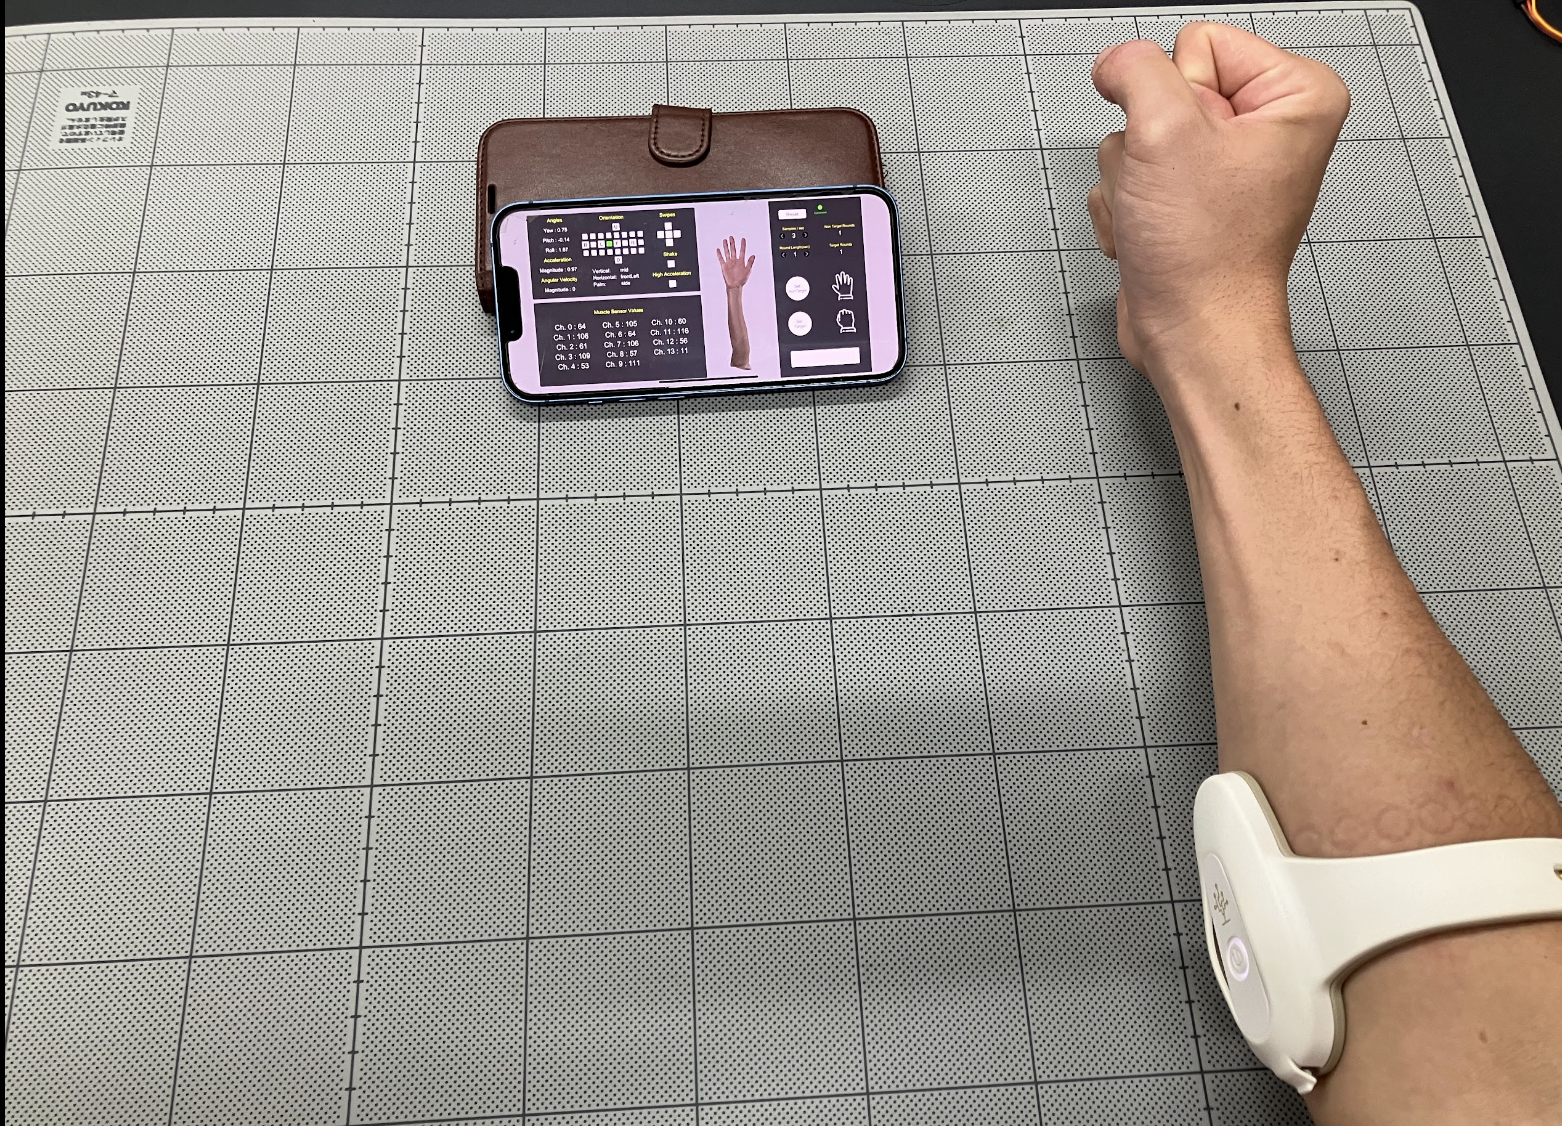
\includegraphics[width = 8cm]{../figs/IMG_5202.PNG}
				\caption{FirstVRの性能評価の参考図}
				\label{fig:firstVRtest}
				\end{figure}
			\item FirstVRの測定\\
				ジェスチャをしていない状態の筋変位センサの値を1回測定し,グーのジェスチャにおけるセンサ値の変化量を5回測定した.
			\item FirstVRのジェスチャ保持特性の検証\\
				ノイズの少なかったsample数を選出し,ジェスチャ状態で手の角度を上下左右に動かした場合のジェスチャ状態の変化を
				動画に撮影して検証する.
		\end{enumerate}

		ノイズの判定方法は実際の腕の動作とアプリケーションの表示が異なる場合にノイズと判定した.
		sample数の選出はノイズの回数が同数だった場合はシミュレータの負荷軽減のためにsample数が少ない方を選出する.

		各実験協力者におけるジェスチャ認識率$G_{r}$は各sample数$D = 11$,ジェスチャ誤判定の回数$m$として,測定回数$s = 5$のとき式\refeq{eq:gestureprobability1}によって求められる.
		\begin{equation}
			\label{eq:gestureprobability1}
			G_{r} = \left( 1-\frac{m}{D \times s} \right) \times 100 \, [%]
		\end{equation}
		また,各sample数におけるジェスチャ認識率$G_{s}$は実験協力者$n = 31$として同様に式\refeq{eq:gestureprobability2}で求められる.
		\begin{equation}
			\label{eq:gestureprobability2}
			G_{s} = \left( 1-\frac{m}{n \times s} \right) \times 100 \, [%]
		\end{equation}
		これらを用いて,ジェスチャの認識率を比較し,最適なsample数の検討を行う.
		
		加えて,FirstVRで筋変位を測定した14チャンネル光変位センサの測定値を用いてジェスチャ認識の精度を確認するため,
		各実験協力者・各sample数ごとの評価指標として総変化量$X$を定める.総変化量の算出は測定回数$s = 5$,チャンネル数$r = 14$としてジェスチャ状態で測定した筋変位センサの値を$M_{{s}{r}}$
		とジェスチャしていない状態の筋変位センサの値$N_{r}$とすると式\refeq{eq:originaldata}と示すことができる.
		この評価指標を用いて各sample数ごとに分散を調べ,最適なsample数の検討を行う.
		\begin{equation}
			\label{eq:originaldata}
			X = \frac{1}{5} \sum_{s = 1}^{5} \sum_{r = 0}^{13} |N_{r} - M_{{s}{r}}|
		\end{equation}
		
	\section{シミュレータの構成}
		Blenderで処理したVHをUnityにインポートし,保持可能オブジェクトを球体,円柱,立方体の3つ用意し,
		大別してPLAYER,STAGE,UIの構成にする.
		\begin{figure}[H]
		\centering
		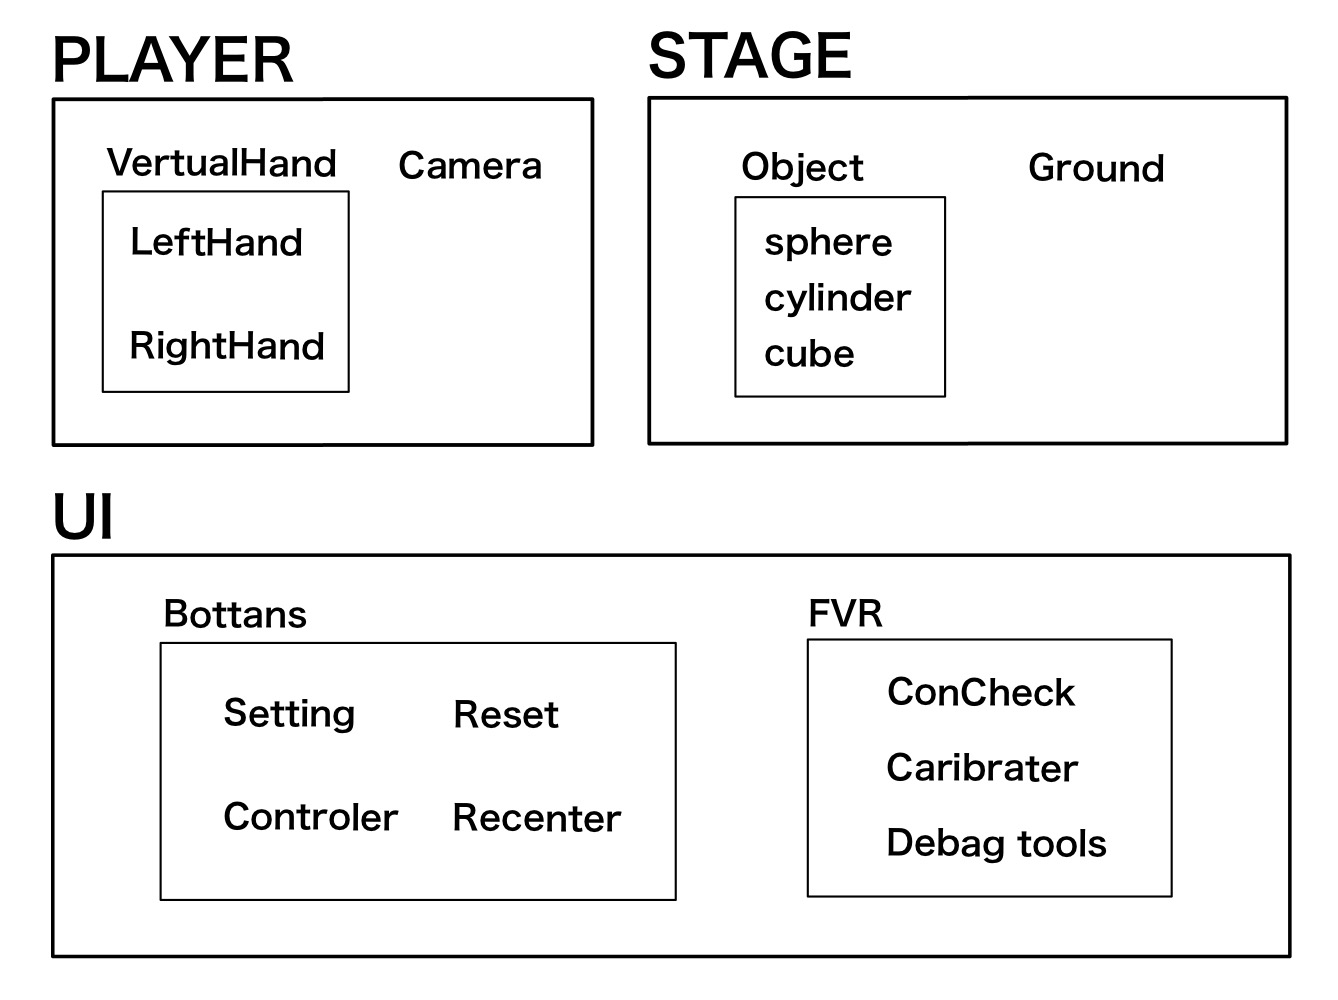
\includegraphics[width = 12cm]{../figs/IMG_0340.JPG}
		\caption{シミュレータ構成図}
		\label{fig:simuraterconst}
		\end{figure}
		playerオブジェクトには右腕オブジェクトのRightArm,左腕オブジェクトのLeftArmとマウスカーソルを追従するtargetオブジェクトを含める.
		また,各Armオブジェクトの掌にはColliderオブジェクトを配置して衝突判定を作成する.

		
	\section{シミュレータの定性評価手法}
		電子工学科学生11名に協力していただき,PC版シミュレータとiOS版シミュレータの2種類の操作説明を説明した後,
		5分程度体験してもらい,各シミュレータにおいて以下の3項目について6段階リッカート尺度を用いた定性評価
		アンケート調査を行う.
		\begin{enumerate}
			\item シミュレータの没入感
			\item インターフェースの操作性
			\item シミュレータの応答性
		\end{enumerate}
		評価点数が高いほどそれぞれの項目において高得点の評価となるように設定し,調査結果に対して分析を行う.

\chapter{研究結果}
	
	\section{VH\,(Virtual Hand)の3Dモデル構成}
		3Dスキャナで取り込んだ左腕3Dモデルと実際の左腕の比較を図\refeq{fig:hikaku}に示す.

		\begin{figure}[H]
		\centering
		\begin{minipage}{0.11\columnwidth}
		\centering
		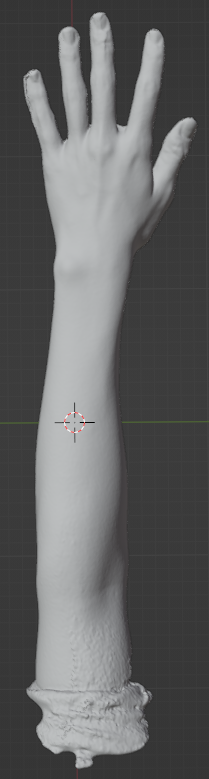
\includegraphics[width = \columnwidth]{../figs/SmoothingBeforALL.png}
		\subcaption{左腕3Dモデル}
		\label{fig:importLeftArm}
		\end{minipage}
		\hspace{0.04\columnwidth}
		\begin{minipage}{0.2\columnwidth}
		\centering
		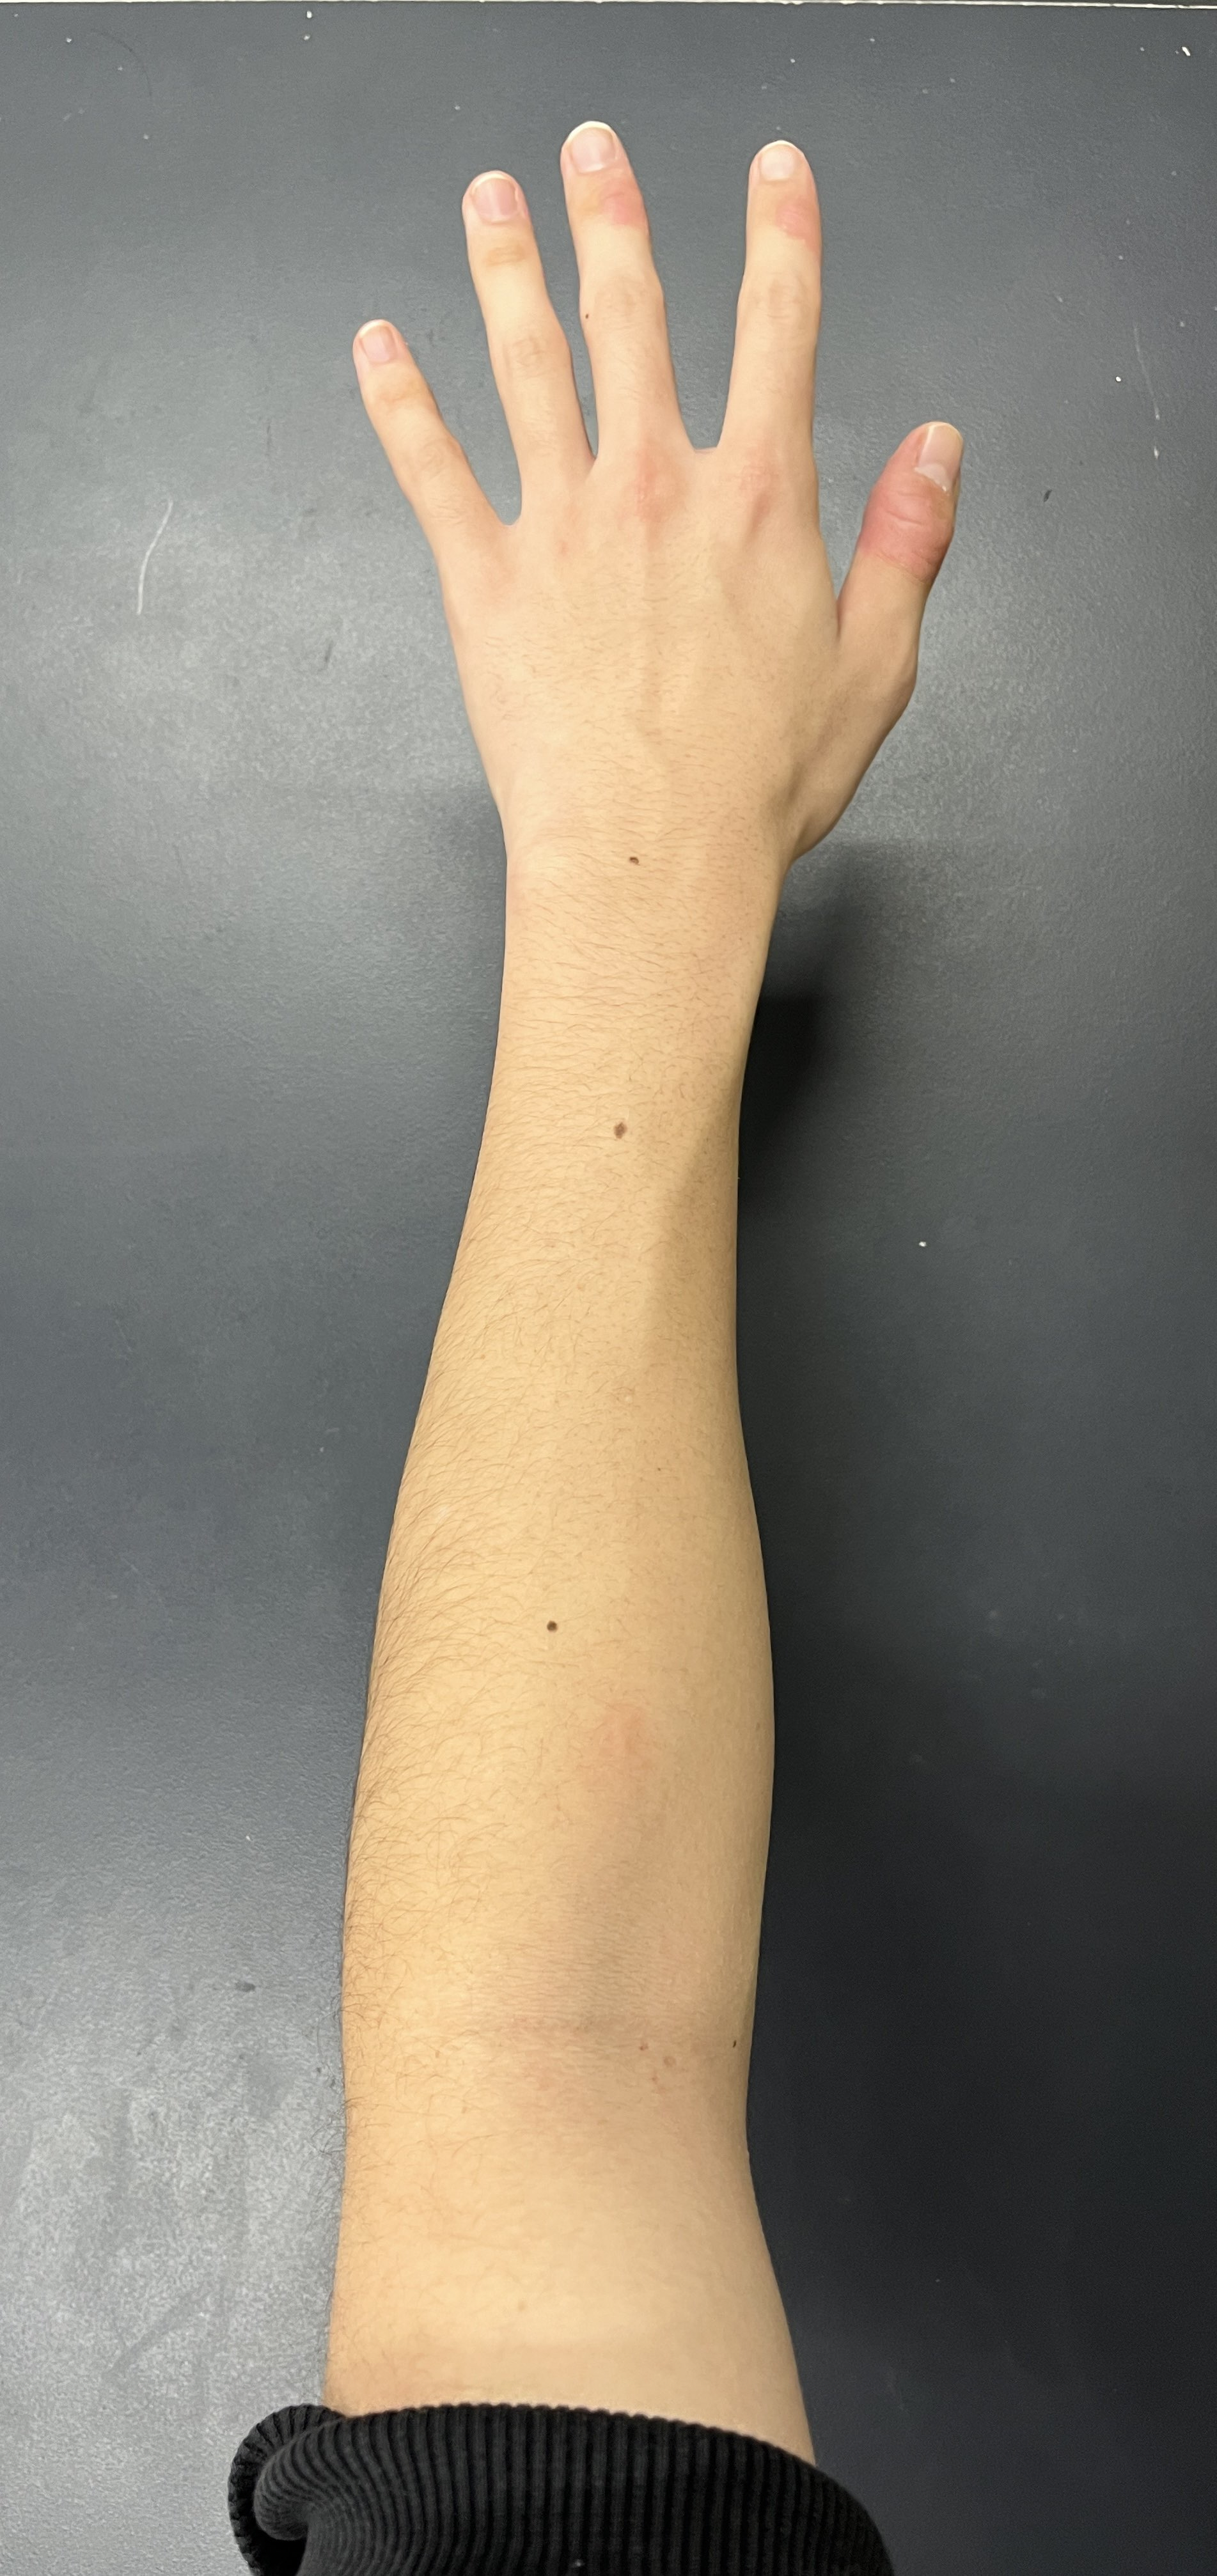
\includegraphics[width = \columnwidth]{../figs/IMG_5145.jpg}
		\subcaption{実際の左腕}
		\label{fig:realLeftArm}
		\vspace{0.12\columnwidth}
		\end{minipage}
		\caption{取り込んだ左腕3Dモデルと実際の左腕の比較}
		\label{fig:hikaku}
		\end{figure}

		\vspace{-10pt}

		実際の左腕と比較して,手の甲の表現や筋の出方の表現がとても精巧に再現されているように感じられる.
		しかし,多少腕周りの太さが細くなっているようにも見られる.また,図\refeq{fig:smoothingbefor}取り込んだ直後の3Dモデルでは撮影
		時のノイズが含まれているため,Blenderのスムージング機能を用いて図\refeq{fig:smoothingafter}のように3Dモデルを平滑化した.

		\begin{figure}[H]
		\centering
		\begin{minipage}{0.3\columnwidth}
		\centering
		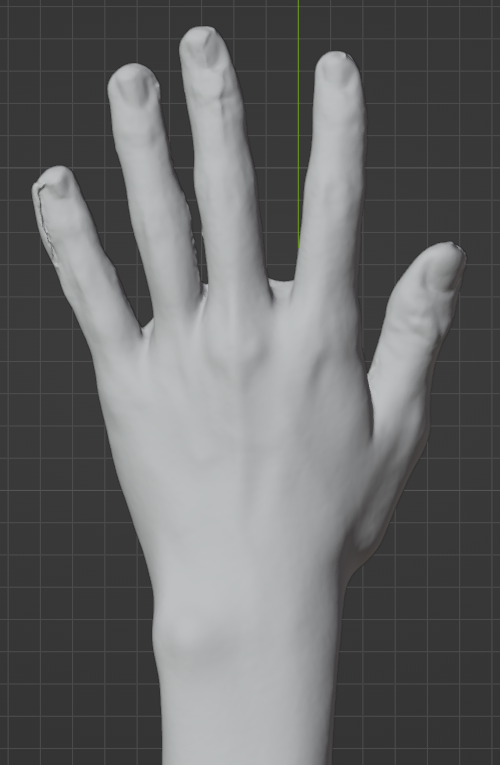
\includegraphics[width = \columnwidth]{../figs/SmoothingBeforRear.png}
		\subcaption{処理前画像}
		\label{fig:smoothingbefor}
		\end{minipage}
		\hspace{0.04\columnwidth}
		\begin{minipage}{0.32\columnwidth}
		\centering
		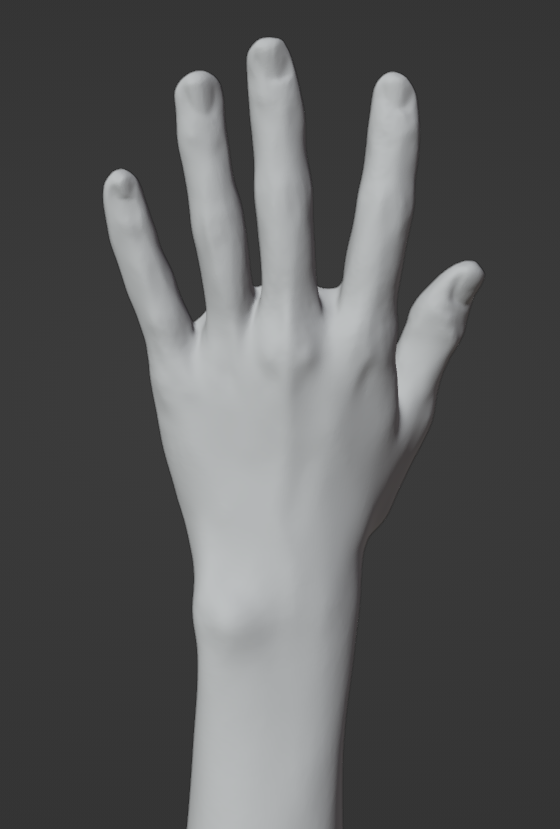
\includegraphics[width = \columnwidth]{../figs/SmoothingAfterRear.png}
		\subcaption{処理後画像}
		\label{fig:smoothingafter}
		\end{minipage}
		\caption{スムージング処理前後の3Dモデル比較}
		\label{fig:smoothing}
		\end{figure}

		図\refeq{fig:smoothing}より,図\refeq{fig:smoothingbefor}では小指や人差し指の先端部分のノイズが
		見られるが,図\refeq{fig:smoothingafter}ではスムージング処理によりノイズが解消されていることが
		わかる.

		また,3DモデルをUnityにインポートする際,オブジェクト保持のアニメーションを作製するためにメッシュ
		の制御を行う必要があるため,図\refeq{fig:meshbone}のようにボーンを配置した.
		\begin{figure}[H]
		\centering
		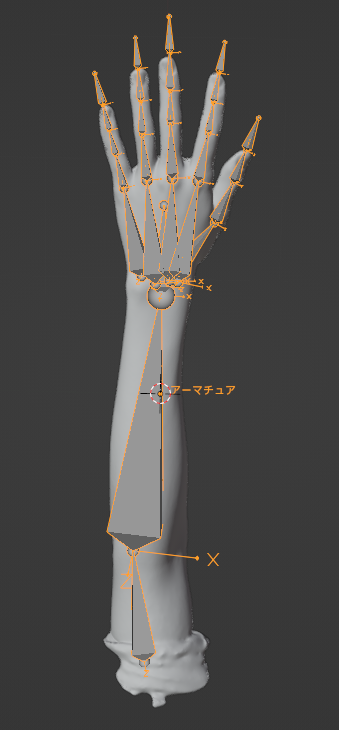
\includegraphics[width = 4cm]{../figs/meshbone.png}
		\caption{ボーン配置図}
		\label{fig:meshbone}
		\end{figure}

		図\refeq{fig:meshbone}より,ボーンは関節を目安に配置しており,各指の先端にはエンドボーンと呼ばれる
		アニメーション制御用のボーンを追加した.このエンドボーンを移動させることで各指のボーン変形
		を自動的に補完するようになっている.

	\section{オブジェクト保持}

		球体,円柱,立方体のオブジェクト3種類の保持アニメーションを図\refeq{fig:spherehold}〜\refeq{fig:cubehold}に示す.

		\begin{figure}[H]
		\centering
		\begin{minipage}{0.4\columnwidth}
		\centering
		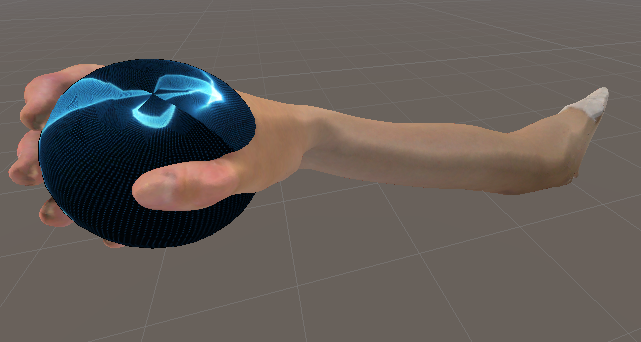
\includegraphics[width = \columnwidth]{../figs/grapsphere_side.png}
		\subcaption{球体保持アニメーション側面図}
		\end{minipage}
		\hspace{0.04\columnwidth}
		\begin{minipage}{0.18\columnwidth}
		\centering
		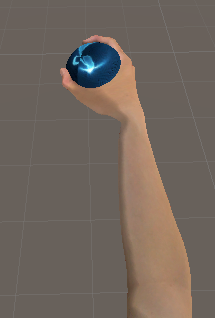
\includegraphics[width = \columnwidth]{../figs/grapsphere_up.png}
		\subcaption{球体保持アニメーション上面図}
		\end{minipage}
		\caption{球体オブジェクトの保持表現}
		\label{fig:spherehold}
		\end{figure}

		\begin{figure}[H]
		\centering
		\begin{minipage}{0.4\columnwidth}
		\centering
		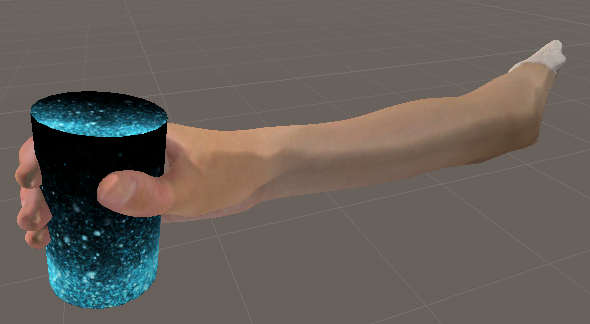
\includegraphics[width = \columnwidth]{../figs/grapcylinder_side.png}
		\subcaption{円柱保持アニメーション側面図}
		\end{minipage}
		\hspace{0.04\columnwidth}
		\begin{minipage}{0.2\columnwidth}
		\centering
		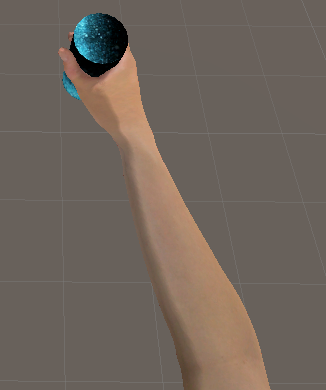
\includegraphics[width = \columnwidth]{../figs/grapcylinder_up.png}
		\subcaption{円柱保持アニメーション上面図}
		\end{minipage}
		\caption{円柱オブジェクトの保持表現}
		\label{fig:cylinderhold}
		\end{figure}

		\begin{figure}[H]
		\centering
		\begin{minipage}{0.4\columnwidth}
		\centering
		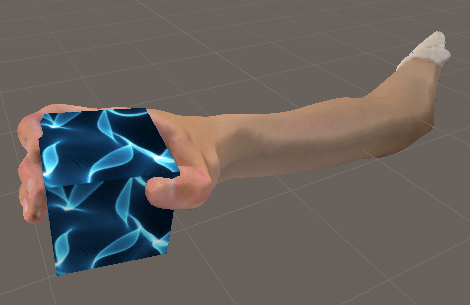
\includegraphics[width = \columnwidth]{../figs/grapcube_side.png}
		\subcaption{立方体保持アニメーション側面図}
		\end{minipage}
		\hspace{0.04\columnwidth}
		\begin{minipage}{0.2\columnwidth}
		\centering
		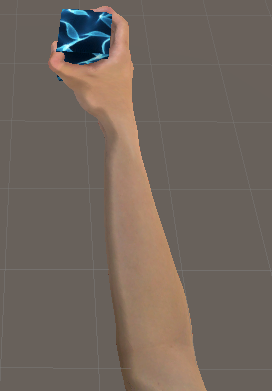
\includegraphics[width = \columnwidth]{../figs/grapcube_up.png}
		\subcaption{立方体保持アニメーション上面図}
		\end{minipage}
		\caption{立方体オブジェクトの保持表現}
		\label{fig:cubehold}
		\end{figure}
		
		オブジェクトが静止状態の場合でも動いている場合でも衝突条件を見たせばオブジェクトを保持することができる.
		実際にボールや水筒などの形の似たものを掴んでいる写真を参考にアニメーションを作製したため,
		かなり現実に近い掴み方をしているように見える.
		しかし,保持アニメーションを行う際,オブジェクトの位置はVHの位置に紐付けられるのだが,オブジェクトの回転までは制御していないので
		円柱や立方体は保持する角度によって指や掌を貫通するような掴み方になる.


		アニメーター構成は図\refeq{fig:Handanimater}のようになっており,

		\begin{figure}[H]
		\centering
		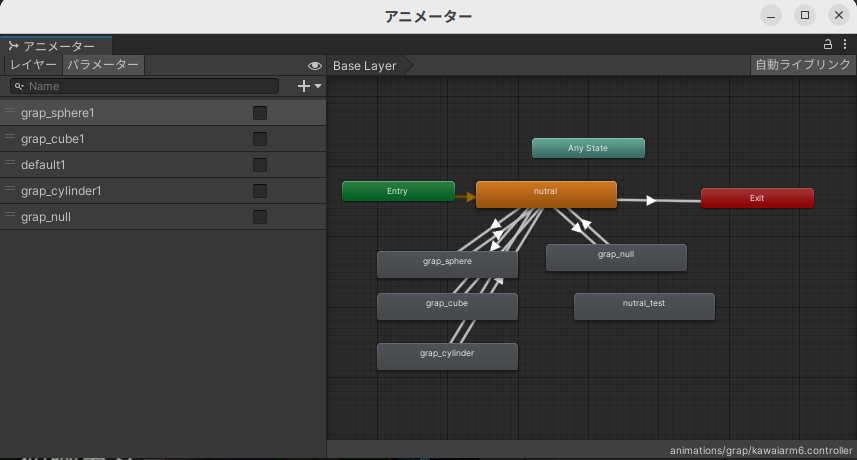
\includegraphics[width = 10cm]{../figs/Handanimater.png}
		\caption{アニメーター構成}
		\label{fig:Handanimater}
		\end{figure}

		各アニメーションの遷移フラグとしてgrap\_sphere1,
		grap\_cylinder1,grap\_cube1を用意した.ジェスチャをしていない状態でnutralというなにもアニメーションをしないクリップをループ再生し続け,
		衝突判定とジェスチャ認識が同時に行われた場合に対応するオブジェクトのフラグを立てて,オブジェクト保持のアニメーションを再生する.

	\section{FirstVRの性能評価}
		FirstVRを装着する様子を図\refeq{fig:FirsrVRfit}に示す.
		\begin{figure}[H]
		\centering
		\includegraphics[width = 10cm]{../figs/IMG_1386.JPG}
		\caption{FirstVR装着方法}
		\label{fig:FirsrVRfit}
		\end{figure}
		机上に5cm四方のグリッド線が描かれたボードを用いて肘の設置店から手首までを測定し,
		その1/4の距離にFirstVRを装着させた.図\refeq{fig:FirstVRevaluation}に測定時の様子を
		示す.

		\begin{figure}[H]
		\centering
		\begin{minipage}{0.45\columnwidth}
		\centering
		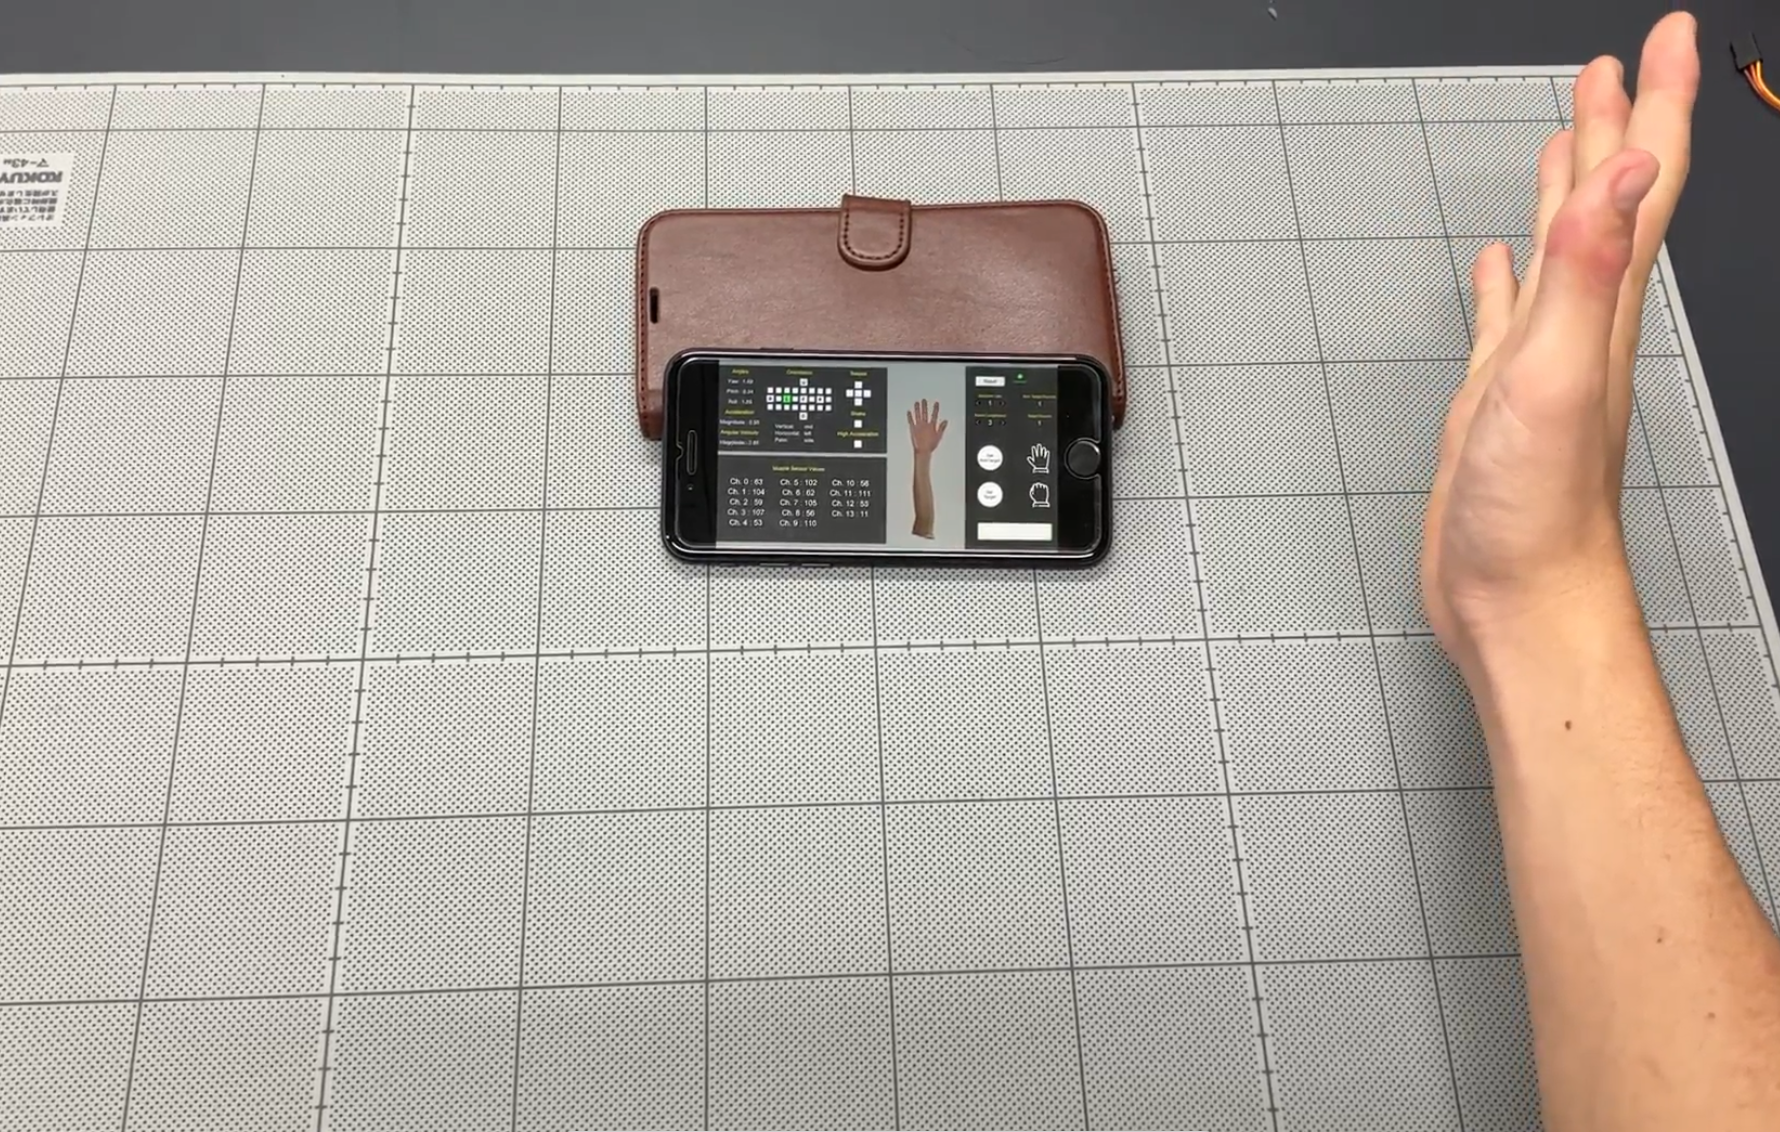
\includegraphics[width = \columnwidth]{../figs/IMG_5200.PNG}
		\end{minipage}
		\hspace{0.04\columnwidth}
		\begin{minipage}{0.45\columnwidth}
		\centering
		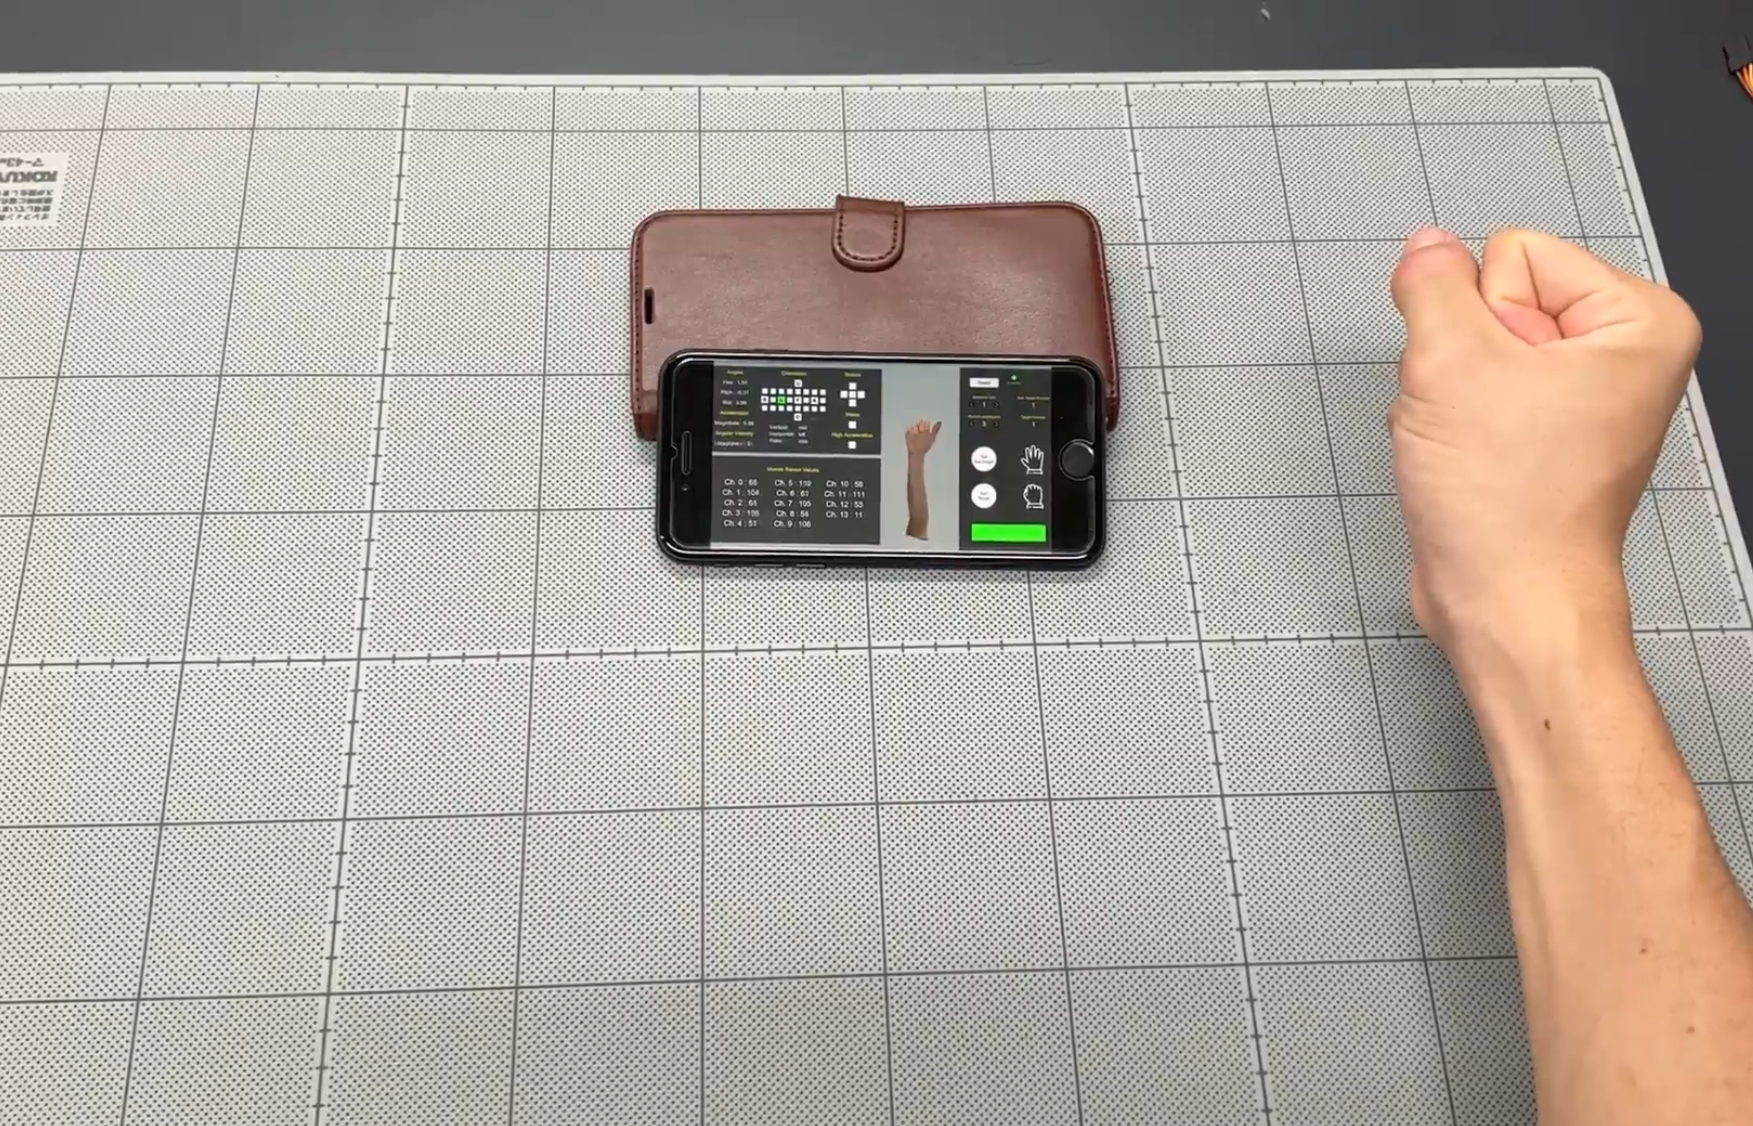
\includegraphics[width = \columnwidth]{../figs/IMG_5201.PNG}
		\end{minipage}
		\caption{FirstVR性能評価の様子}
		\label{fig:FirstVRevaluation}
		\end{figure}
		
		図\refeq{fig:FirstVRevaluation}のようにジェスチャ状態を1回,ジェスチャしていない状態を5回
		測定し,それを各sample数で繰り返した.全員分のデータは記載することができないため付録にあるQRコードから
		FVRDataFilesを開いてもらうと各実験協力者のデータが閲覧できるようになっている.
		データの傾向としては,ジェスチャ状態の登録の際,強く握りすぎない方がジェスチャ認識のノイズが低減した.

\clearpage

		FirstVRの性能評価用アプリケーションの構成を図\refeq{fig:FirstVRapplication}に示す.
		\begin{figure}[H]
		\centering
		\begin{minipage}{0.7\columnwidth}
		\centering
		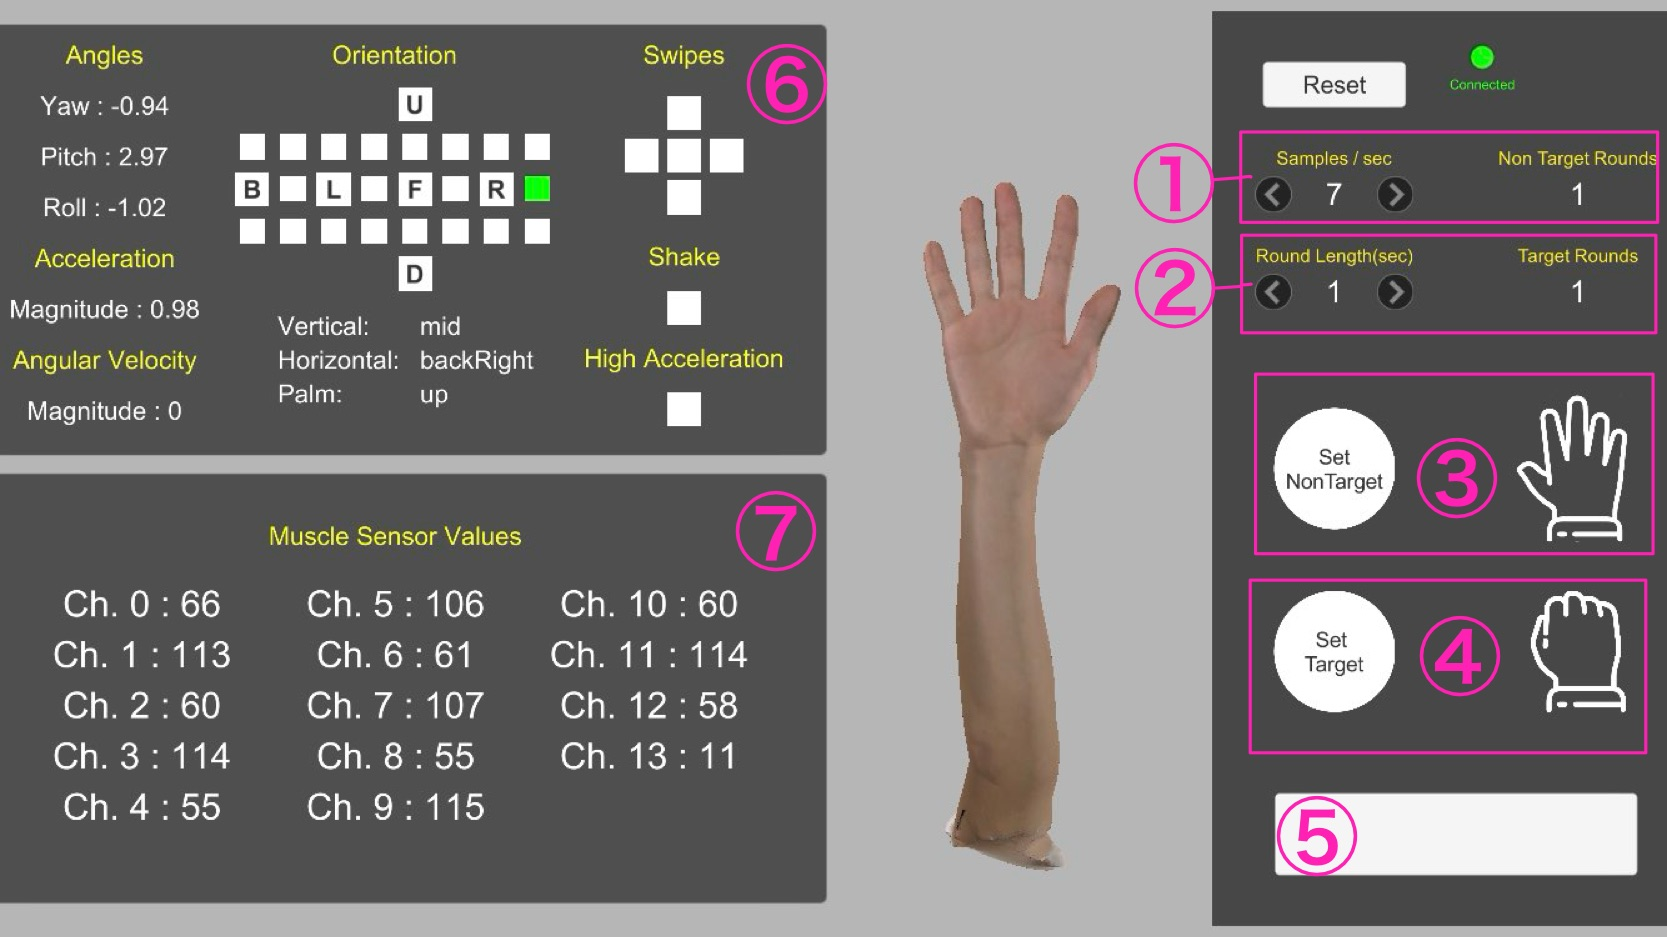
\includegraphics[width = \columnwidth]{../figs/IMG_0345.JPG}
		\subcaption{ジェスチャ未判定時}
		\label{fig:FVRnocalibration}
		\end{minipage}
		\hspace{0.04\columnwidth}
		\begin{minipage}{0.7\columnwidth}
		\centering
		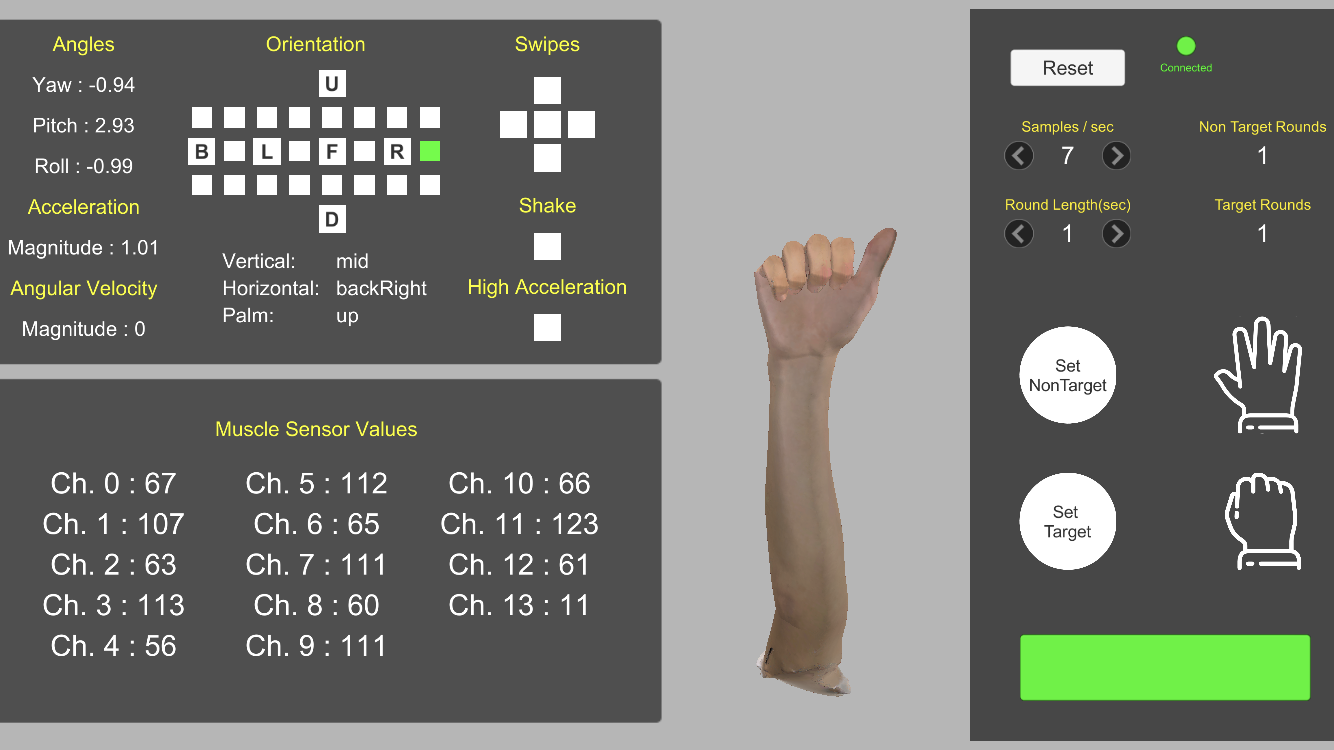
\includegraphics[width = \columnwidth]{../figs/IMG_1867.PNG}
		\subcaption{ジェスチャ判定時}
		\end{minipage}
		\caption{FirstVR性能評価用アプリケーションの構成}
		\label{fig:FirstVRapplication}
		\end{figure}
		図\refeq{fig:FVRnocalibration}の①で学習させるsample数を設定でき,②では学習時間を設定することができる.
		また,ジェスチャしていない状態を学習させるときは③のボタン,ジェスチャ状態を学習させるときは④のボタンで
		学習させることができる.学習が完了すると,①と②の右側のカウントが増えていく.
		FirstVRの性能評価の際は簡易のために学習時間を1に固定してsample数のみを変化させた.
		ジェスチャ判定時には⑤のバーが白色から緑色に変化するため,ジェスチャをした瞬間の筋変位センサの値を測定し,
		そのタイミングでバーの色が変化していなければジェスチャ認識ができていないものとした.
		⑥は性能評価に用いなかったが,トラッキングのデータを取ることができ,手のヨー,ピッチ,ロールの値やスワイプ方向の取得が可能である.
		⑦はFirstVR裏面にある筋変位センサの各チャンネル毎の測定値を見ることができる.
		この値を用いて,最適sample数の選定を行った.

\clearpage

		各実験協力者におけるジェスチャ認識率を表\refeq{tab:gestureprobability1}に示す.
		\begin{table}[H]
		\begin{center}
		\caption{各実験協力者におけるジェスチャ認識率}
		\label{tab:gestureprobability1}
		\begin{tabular}{cSS}\Hline
		Person& 誤検知回数 [回] & ジェスチャ認識率 [%] \\ \hline
		1 & 4 & 92.73 \\
		2 & 0 & 100.00 \\
		3 & 1 & 98.18 \\
		4 & 3 & 94.55 \\
		5 & 0 & 100.00 \\
		6 & 3 & 94.55 \\
		7 & 0 & 100.00 \\
		8 & 0 & 100.00 \\
		9 & 4 & 92.73 \\
		10 & 17 & 69.09 \\
		11 & 0 & 100.00 \\
		12 & 0 & 100.00 \\
		13 & 0 & 100.00 \\
		14 & 16 & 70.91 \\
		15 & 0 & 100.00 \\
		16 & 0 & 100.00 \\
		17 & 2 & 96.36 \\
		18 & 3 & 94.55 \\
		19 & 27 & 50.91 \\
		20 & 1 & 98.18 \\
		21 & 3 & 94.55 \\
		22 & 1 & 98.18 \\
		23 & 0 & 100.00 \\
		24 & 5 & 90.91 \\
		25 & 7 & 87.27 \\
		26 & 1 & 98.18 \\
		27 & 0 & 100.00 \\
		28 & 2 & 96.36 \\
		29 & 1 & 98.18 \\
		30 & 14 & 74.55 \\
		31 & 4 & 92.73 \\ \Hline
		\end{tabular}
		\end{center}
		\end{table}

		表\refeq{tab:gestureprobability1}より,ジェスチャ誤検知の回数が極端に多い場合とほとんど誤検知がないというように分布していることがわかる.
		また,10回以上誤検知が起きている実験協力者のデータでは特定のsample数によらずに誤検知が発生しているため,sample数によるジェスチャ認識率のデータ
		含めてしまうとノイズによってデータが正しく求められないため除外した.

		各sample数ごとのジェスチャ認識率を表\refeq{tab:gestureprobability2}に示す.
		\begin{table}[H]
		\begin{center}
		\caption{sample数ごとのジェスチャ認識率}
		\label{tab:gestureprobability2}
		\begin{tabular}{cSS}\Hline
			sample数& 誤検知回数 [回] & ジェスチャ認識率 [%] \\ \hline
			7 & 9 & 93.33 \\
			10 & 2 & 98.52 \\
			20 & 4 & 97.04 \\
			30 & 3 & 97.78 \\
			40 & 5 & 96.30 \\
			50 & 6 & 95.56 \\
			60 & 6 & 95.56 \\
			70 & 2 & 98.52 \\
			80 & 0 & 100.00 \\
			90 & 5 & 96.30 \\
			100 & 3 & 97.78 \\ \hline
			合計 & 45 & 96.97 \\ \Hline
		\end{tabular}
		\end{center}
		\end{table}
		表\refeq{tab:gestureprobability2}より,最低値93.33%,最高値100%のジェスチャ認識率だった.
		したがって,96.66 ± 3.34%の範囲で変動していることがわかる.
		しかし,どのsample数においてもジェスチャの認識率が90%を上回っているため,
		このデータからどのsample数が最適か判定できなかった.

\clearpage
		FirstVRのsample数における総変化量を表\refeq{tab:FVRdata}に示す.
		\begin{table}[H]
		\begin{center}
		\caption{各実験協力者におけるsample数ごとの総変化量一覧}
		\label{tab:FVRdata}
		\begin{tabular}{c|ccccccccccc} \Hline
			Person/sample & 7 & 10 & 20 & 30 & 40 & 50 & 60 & 70 & 80 & 90 & 100 \\ \hline
			1 & 44.4 & 25.6 & 21.8 & 19.4 & 12.2 & 12.6 & 13.4 & 22.4 & 8.2 & 11.8 & 27.2 \\
			2 & 37.0 & 23.4 & 30.2 & 17.2 & 27.2 & 31.8 & 45.4 & 26.2 & 29.4 & 19.2 & 18.2 \\
			3 & 23.4 & 20.2 & 28.4 & 20.6 & 21.8 & 30.4 & 17.2 & 23.6 & 39.0 & 17.4 & 22.0 \\
			4 & 49.0 & 69.8 & 108.8 & 100.6 & 78.0 & 62.2 & 61.4 & 40.8 & 60.6 & 36.6 & 37.6 \\
			5 & 38.2 & 53.2 & 51.2 & 34.6 & 35.4 & 43.6 & 46.6 & 48.2 & 47.4 & 32.0 & 37.6 \\
			6 & 31.8 & 15.6 & 17.6 & 38.4 & 23.2 & 23.4 & 32.0 & 37.8 & 14.8 & 22.4 & 22.0 \\
			7 & 69.2 & 44.8 & 57.0 & 25.8 & 33.2 & 39.6 & 23.0 & 33.6 & 53.8 & 29.8 & 40.0 \\
			8 & 67.0 & 66.0 & 55.4 & 65.0 & 67.0 & 78.6 & 93.6 & 59.0 & 66.8 & 59.4 & 65.4 \\
			9 & 44.4 & 25.6 & 21.8 & 19.4 & 12.2 & 12.6 & 13.4 & 22.4 & 8.2 & 11.8 & 27.2 \\
			10 & 20.8 & 13.8 & 15.4 & 16.4 & 13.2 & 17.8 & 43.8 & 17.6 & 12.0 & 83.6 & 14.4 \\
			11 & 24.8 & 22.8 & 26.2 & 21.0 & 27.8 & 48.8 & 41.2 & 15.6 & 23.2 & 14.2 & 19.4 \\
			12 & 34.2 & 29.8 & 19.8 & 25.8 & 24.0 & 18.2 & 32.4 & 25.4 & 35.4 & 35.6 & 25.2 \\
			13 & 20.6 & 17.4 & 21.6 & 29.0 & 19.0 & 22.8 & 27.6 & 32.2 & 56.8 & 44.0 & 31.2 \\
			14 & 19.8 & 22.0 & 11.6 & 10.0 & 16.8 & 17.4 & 12.4 & 17.6 & 21.6 & 15.8 & 11.4 \\
			15 & 50.8 & 58.4 & 51.2 & 56.6 & 67.4 & 37.6 & 45.8 & 52.4 & 51.6 & 59.6 & 56.2 \\
			16 & 35.2 & 50.2 & 62.6 & 36.4 & 27.2 & 39.6 & 38.8 & 43.4 & 45.4 & 52.4 & 48.8 \\
			17 & 49.4 & 42.2 & 41.2 & 36.4 & 49.4 & 34.4 & 33.2 & 34.4 & 22.2 & 13.8 & 36.0 \\
			18 & 23.8 & 26.8 & 36.2 & 38.0 & 28.0 & 35.2 & 34.0 & 24.4 & 29.2 & 39.6 & 25.8 \\
			19 & 33.6 & 11.8 & 10.4 & 16.8 & 17.8 & 11.0 & 19.4 & 13.6 & 24.4 & 13.2 & 9.6 \\
			20 & 32.6 & 36.4 & 33.0 & 17.6 & 22.6 & 26.8 & 32.2 & 25.2 & 20.8 & 30.4 & 13.8 \\
			21 & 32.8 & 42.6 & 36.6 & 30.6 & 26.4 & 41.4 & 32.6 & 20.2 & 25.0 & 15.8 & 17.6 \\
			22 & 42.2 & 27.6 & 37.8 & 33.8 & 39.2 & 50.0 & 34.6 & 38.0 & 38.8 & 26.8 & 24.2 \\
			23 & 51.8 & 40.4 & 44.0 & 44.6 & 41.4 & 39.2 & 42.8 & 38.4 & 41.6 & 43.0 & 30.0 \\
			24 & 38.0 & 30.6 & 38.2 & 35.6 & 23.8 & 20.4 & 24.4 & 24.2 & 22.6 & 30.6 & 16.8 \\
			25 & 25.2 & 33.0 & 32.0 & 23.8 & 28.0 & 20.0 & 31.4 & 13.6 & 19.6 & 19.4 & 21.2 \\
			26 & 39.8 & 32.8 & 30.2 & 38.2 & 34.8 & 22.6 & 30.4 & 24.0 & 24.0 & 12.6 & 20.6 \\
			27 & 68.8 & 78.0 & 50.4 & 51.6 & 44.2 & 50.8 & 40.0 & 48.2 & 46.4 & 48.8 & 62.0 \\
			28 & 20.4 & 29.8 & 40.6 & 45.0 & 23.8 & 25.2 & 27.4 & 39.0 & 25.2 & 28.8 & 39.6 \\
			29 & 32.6 & 29.8 & 21.6 & 19.0 & 22.4 & 17.6 & 21.2 & 28.2 & 41.4 & 35.6 & 20.8 \\
			30 & 23.2 & 8.0 & 13.6 & 23.2 & 21.2 & 25.4 & 24.0 & 12.6 & 16.0 & 24.4 & 17.8 \\
			31 & 44.4 & 25.6 & 21.8 & 19.4 & 12.2 & 12.6 & 13.4 & 22.4 & 8.2 & 11.8 & 27.2 \\ \hline
			標本分散&189.9 & 287.3 & 375.3 & 315.9 & 259.9 & 241.7 & 252.4 & 143.3 & 256.2 & 290.8 & 196.0 \\ \Hline
			
		\end{tabular}
		\end{center}
		\end{table}

		総変化量が10前後の数値ではFirstVRがジェスチャに対してほとんど応答していなかった.
		この結果を用いて,同sample数における実験協力者ごとの数値の分散が少ないsample数が最適とした.

\clearpage
		図\refeq{fig:FVRdata}に各sample数の分散を示す.

		\begin{figure}[H]
		\centering
		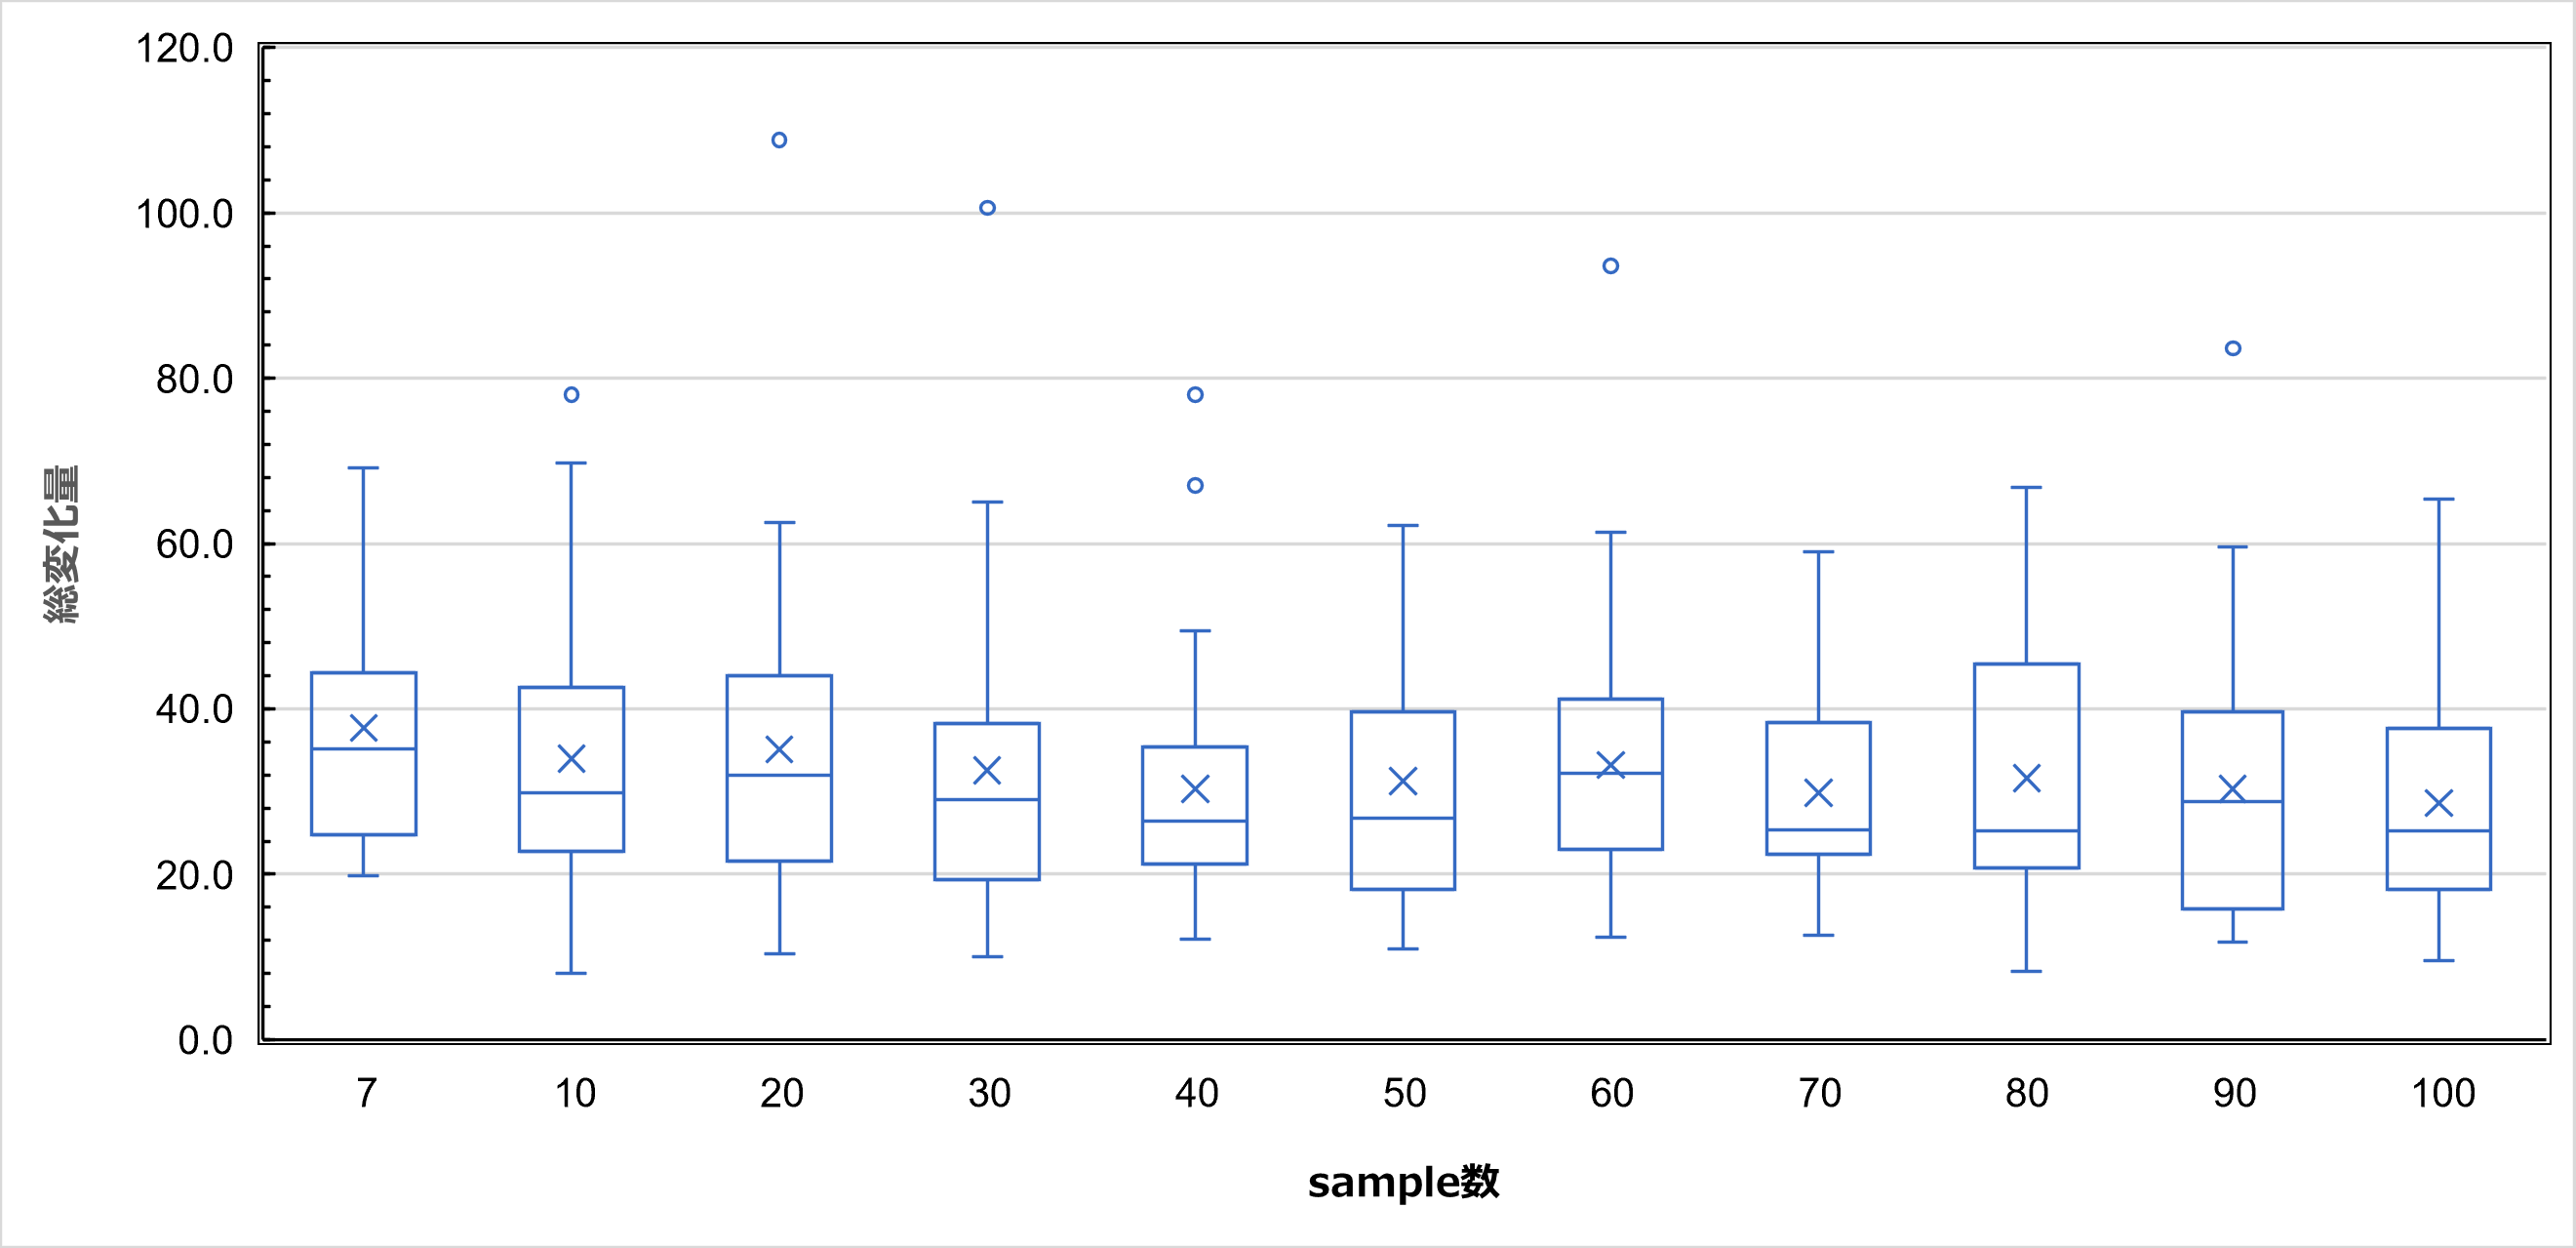
\includegraphics[width = 14cm]{../figs/FVRALL.png}
		\caption{sample数ごとの総変化量分散}
		\label{fig:FVRdata}
		\end{figure}

		図\refeq{fig:FVRdata}より,標本分散はsample70が最も小さく,次いでsample7が分散が少なくなっていることがわかる.
		ここで,sample数7,70,100以外のデータは分散がこの3種類よりも比較的大きく,外れ値も含んでいるため,安定して動作していると考えにくい.
		また,この3種類の中で最もシミュレータに対する負荷が小さいデータとしてsample7を選定した.

	\section{シミュレータの構成}

		\begin{figure}[H]
		\centering
		\begin{minipage}{0.7\columnwidth}
		\centering
		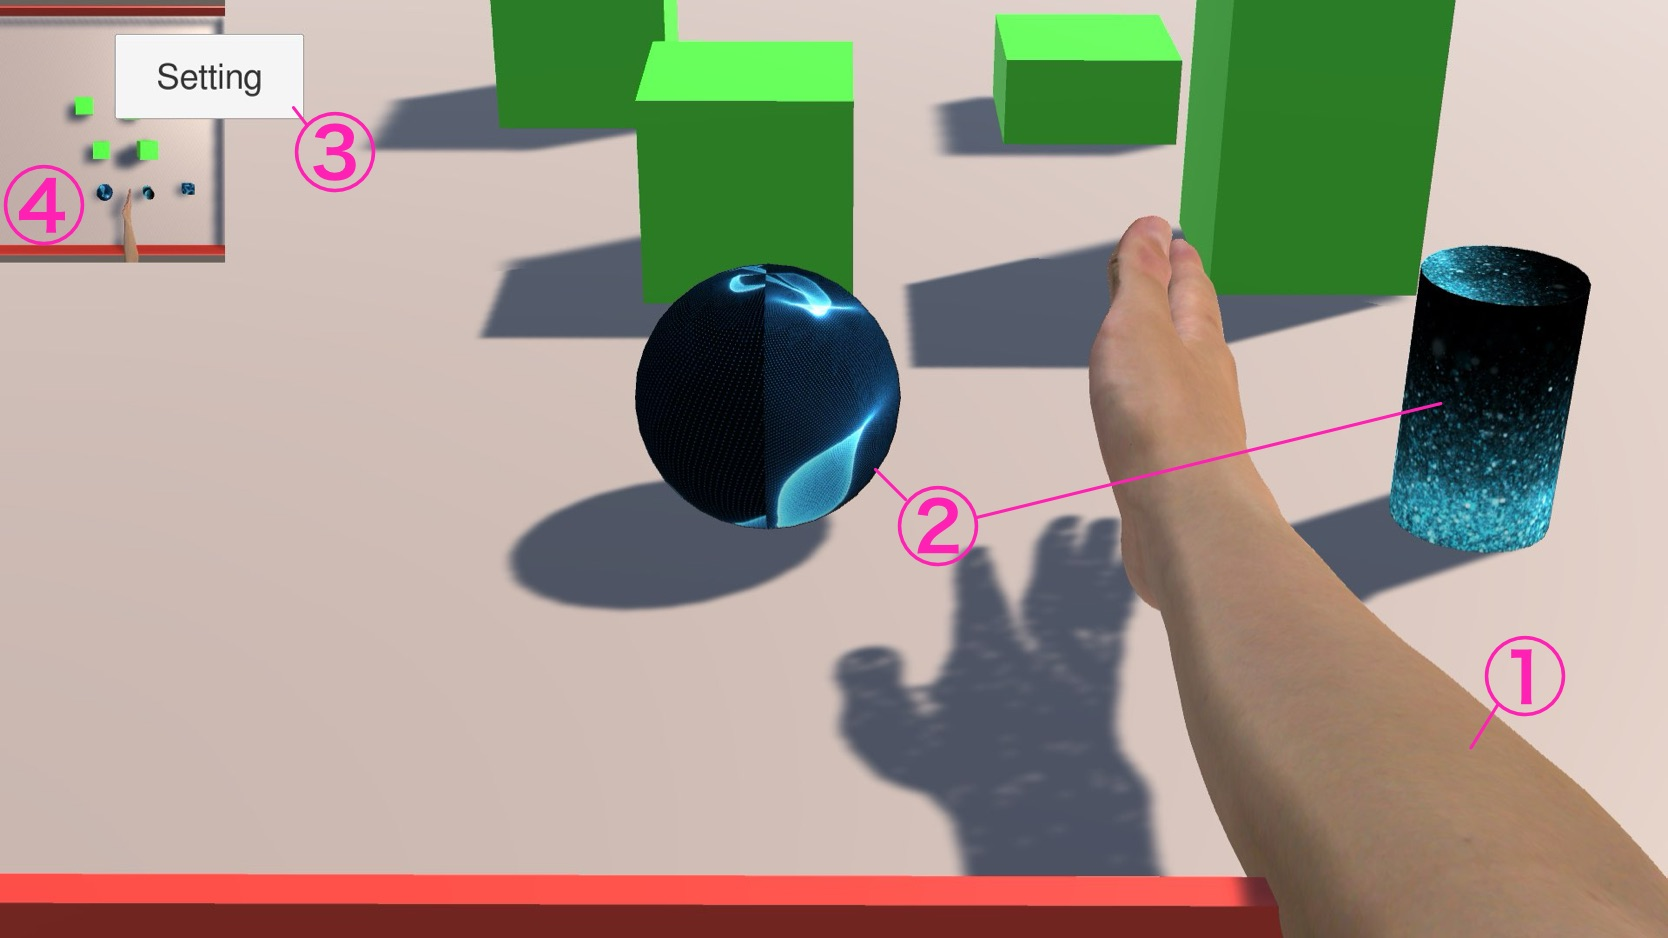
\includegraphics[width = \columnwidth]{../figs/IMG_0341.JPG}
		\subcaption{通常時の画面構成}
		\end{minipage}
		\hspace{0.04\columnwidth}
		\begin{minipage}{0.7\columnwidth}
		\centering
		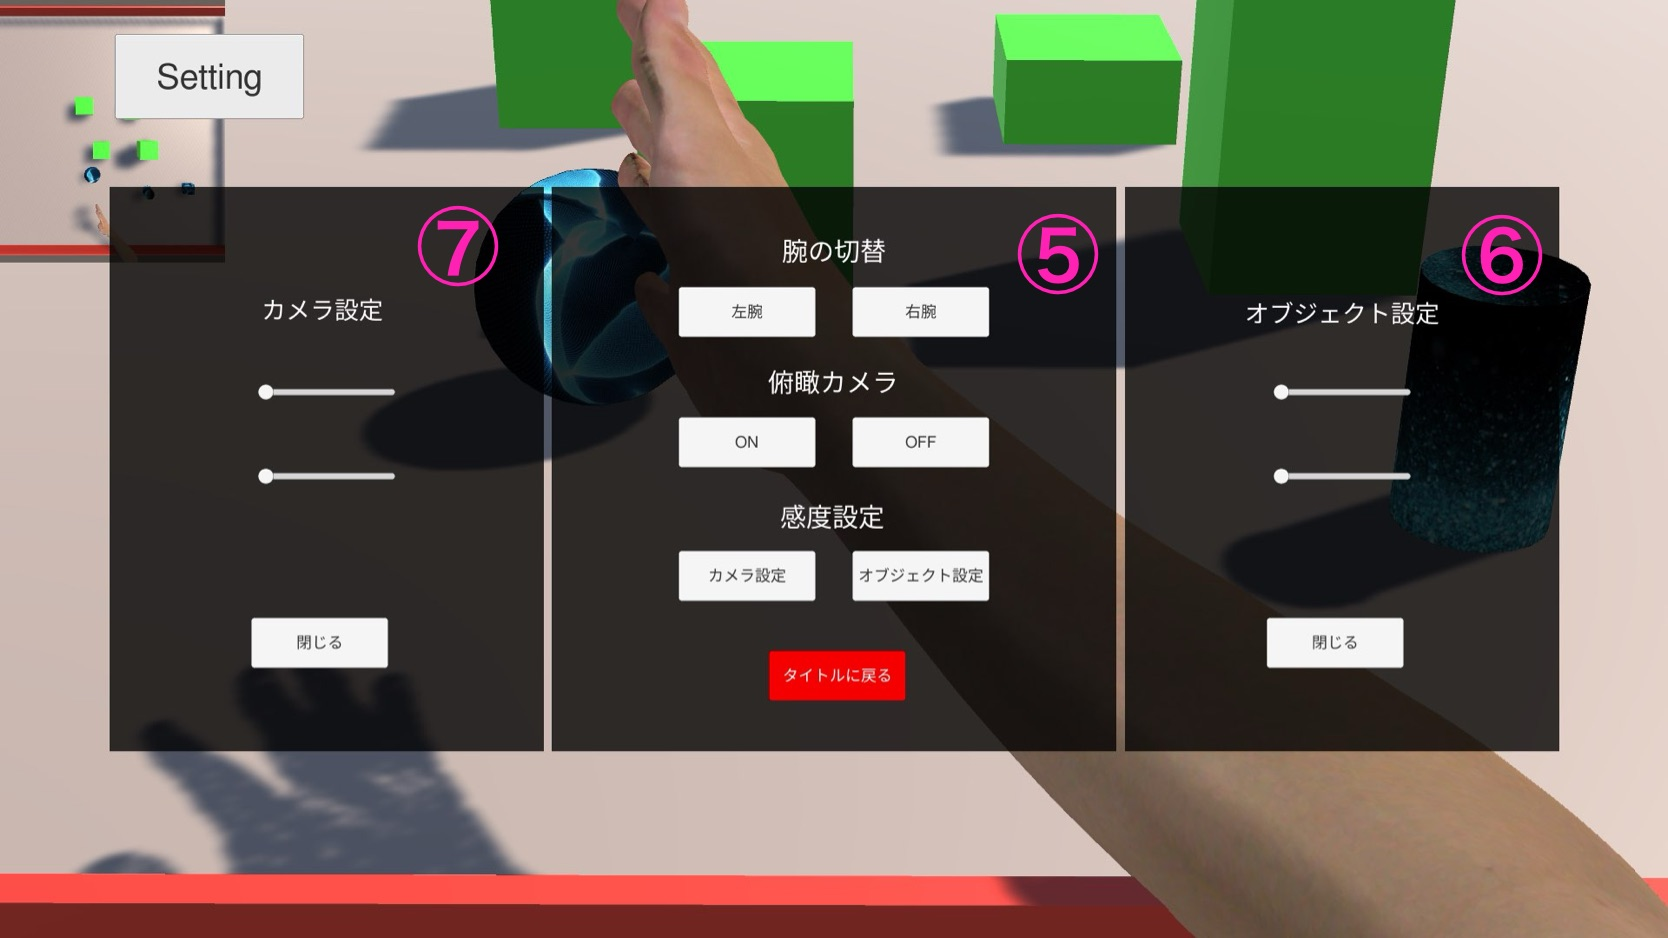
\includegraphics[width = \columnwidth]{../figs/IMG_0342.JPG}
		\subcaption{メニュー起動時の画面構成}
		\end{minipage}
		\caption{PC版シミュレータの実行画面}
		\end{figure}

		\begin{figure}[H]
		\centering
		\begin{minipage}{0.7\columnwidth}
		\centering
		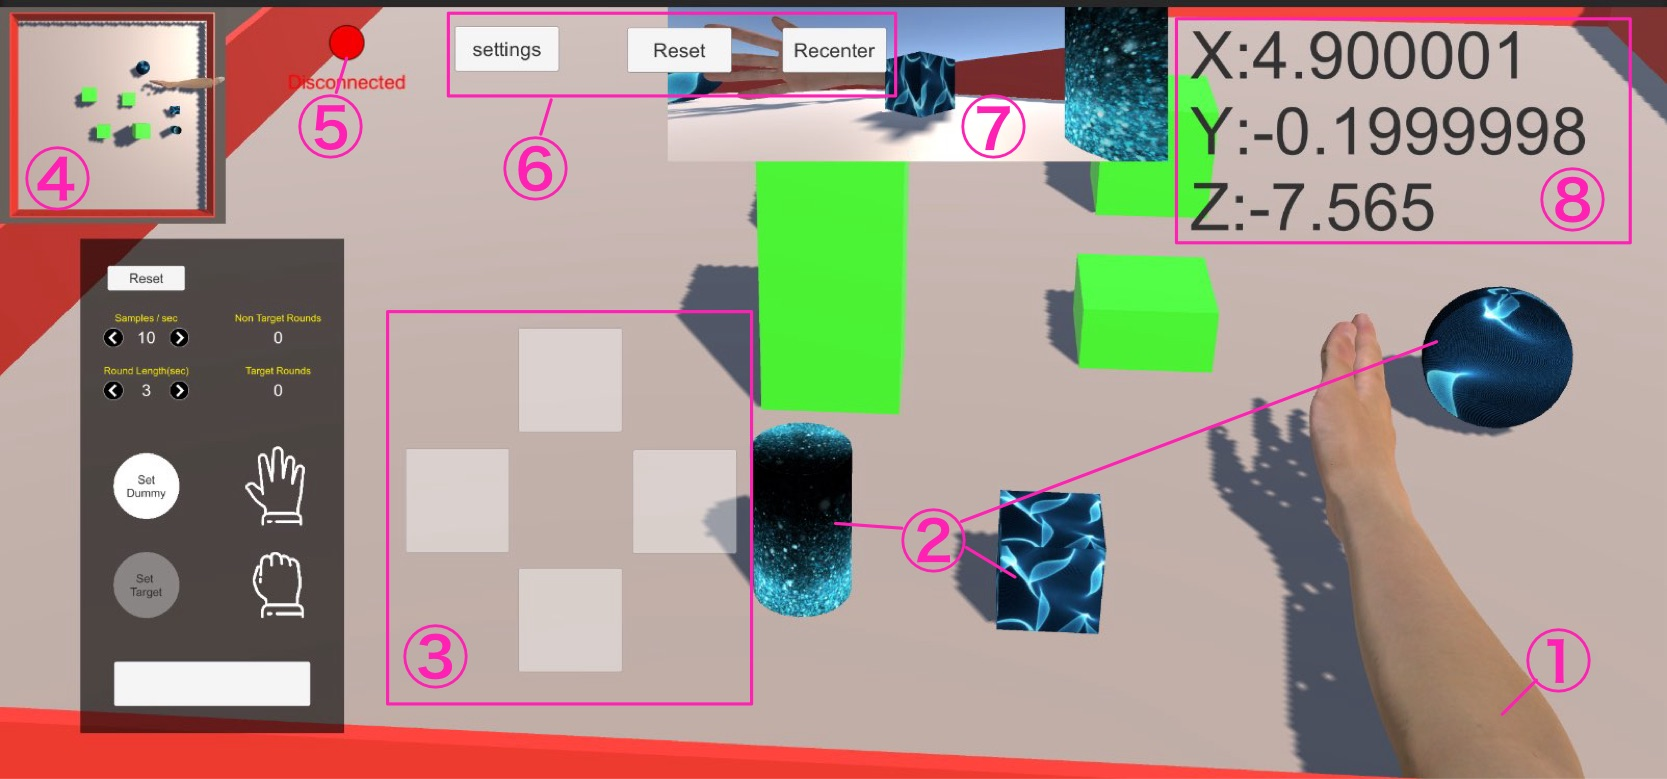
\includegraphics[width = \columnwidth]{../figs/IMG_0344.JPG}
		\subcaption{通常時の画面構成}
		\end{minipage}
		\hspace{0.04\columnwidth}
		\begin{minipage}{0.7\columnwidth}
		\centering
		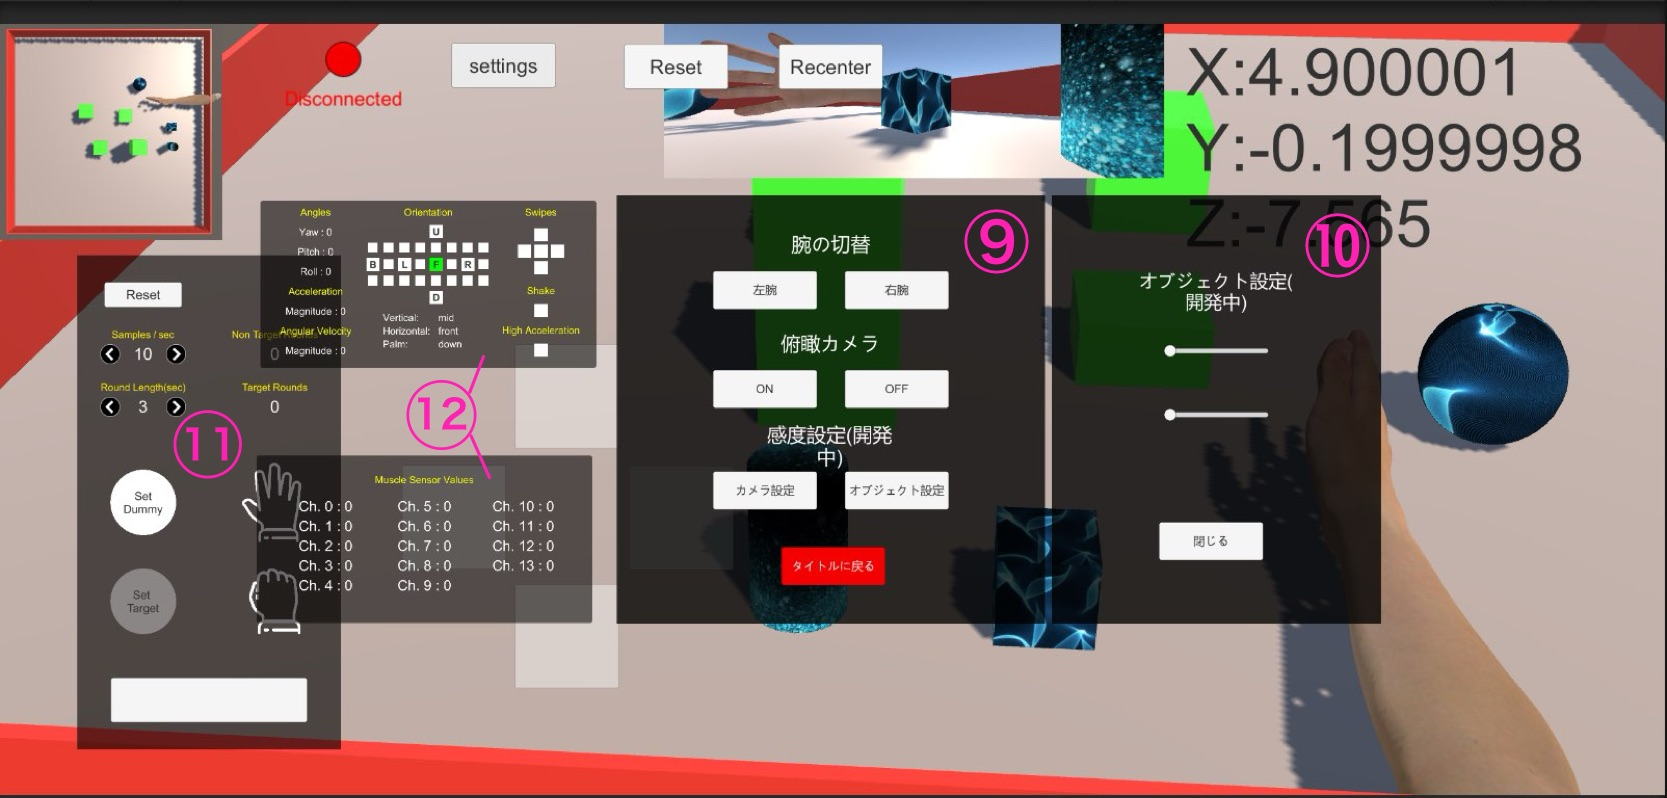
\includegraphics[width = \columnwidth]{../figs/IMG_0343.JPG}
		\subcaption{メニュー起動時の画面構成}
		\end{minipage}
		\caption{iOS版シミュレータの実行画面}
		\label{fig:iOSsimulate}
		\end{figure}

	\section{シミュレータの定性評価}

		\begin{figure}[H]
		\centering
		\begin{minipage}{0.4\columnwidth}
		\centering
		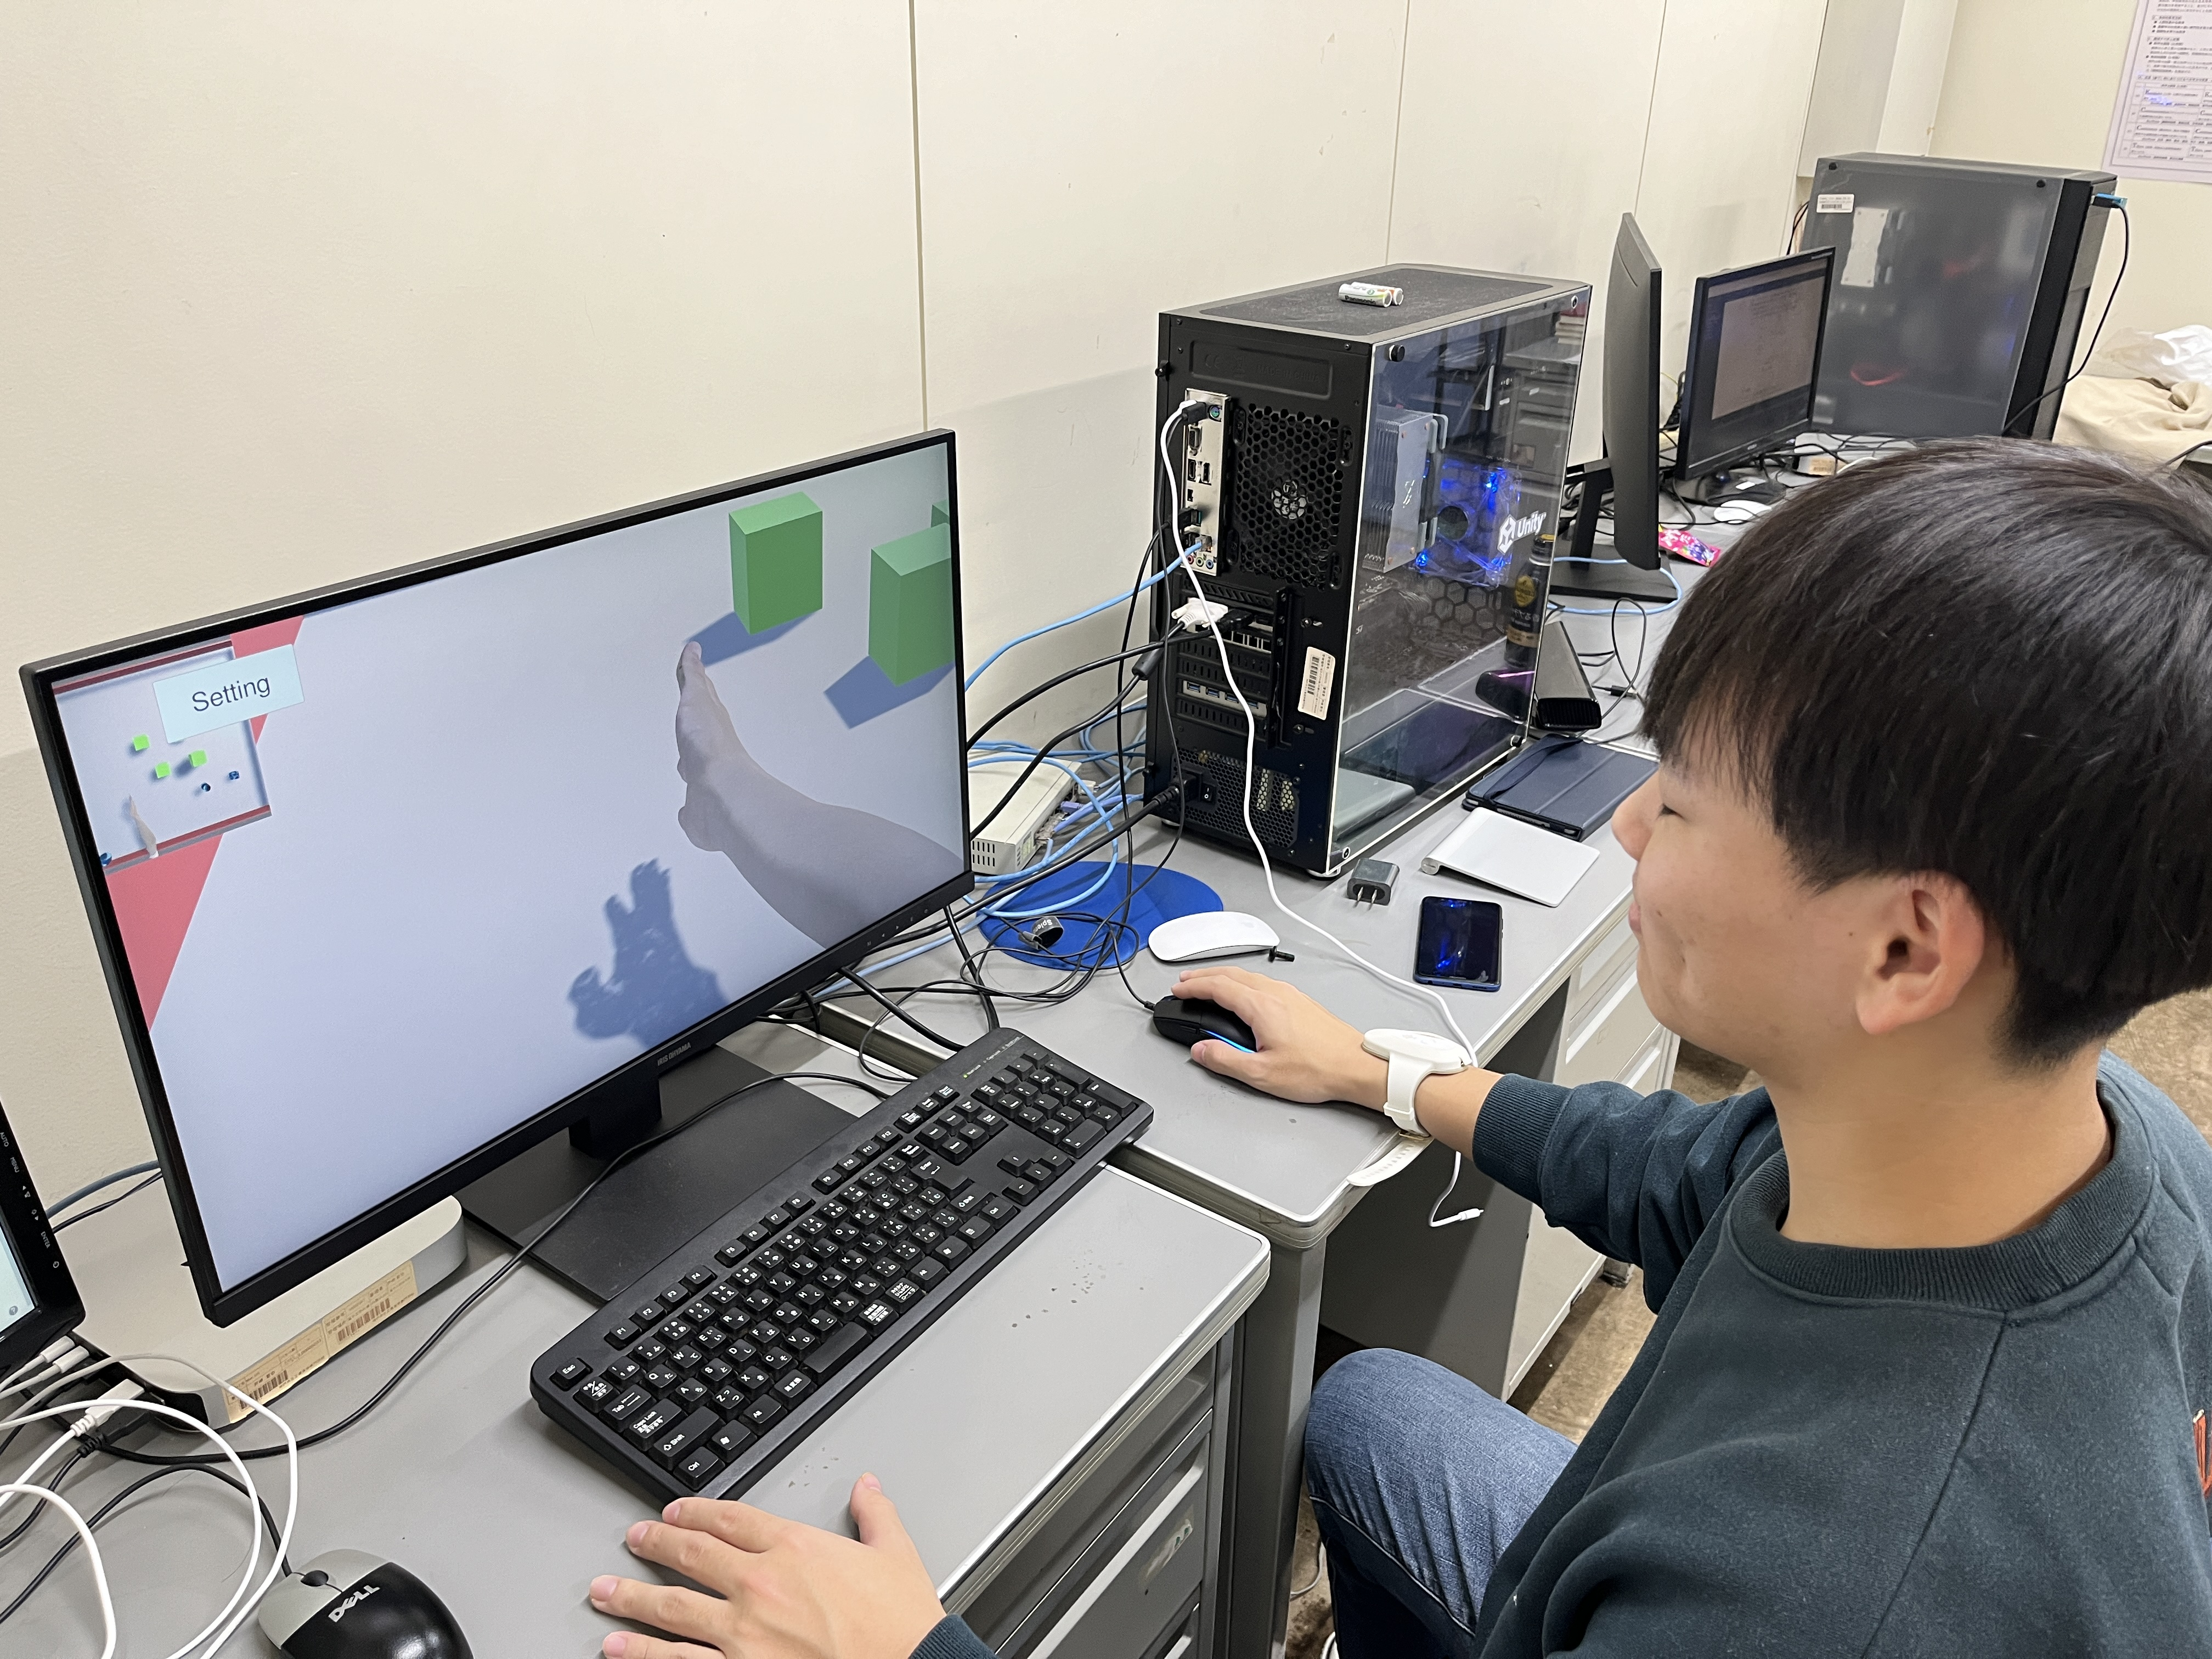
\includegraphics[width = \columnwidth]{../figs/IMG_5132.JPG}
		\end{minipage}
		\hspace{0.04\columnwidth}
		\begin{minipage}{0.4\columnwidth}
		\centering
		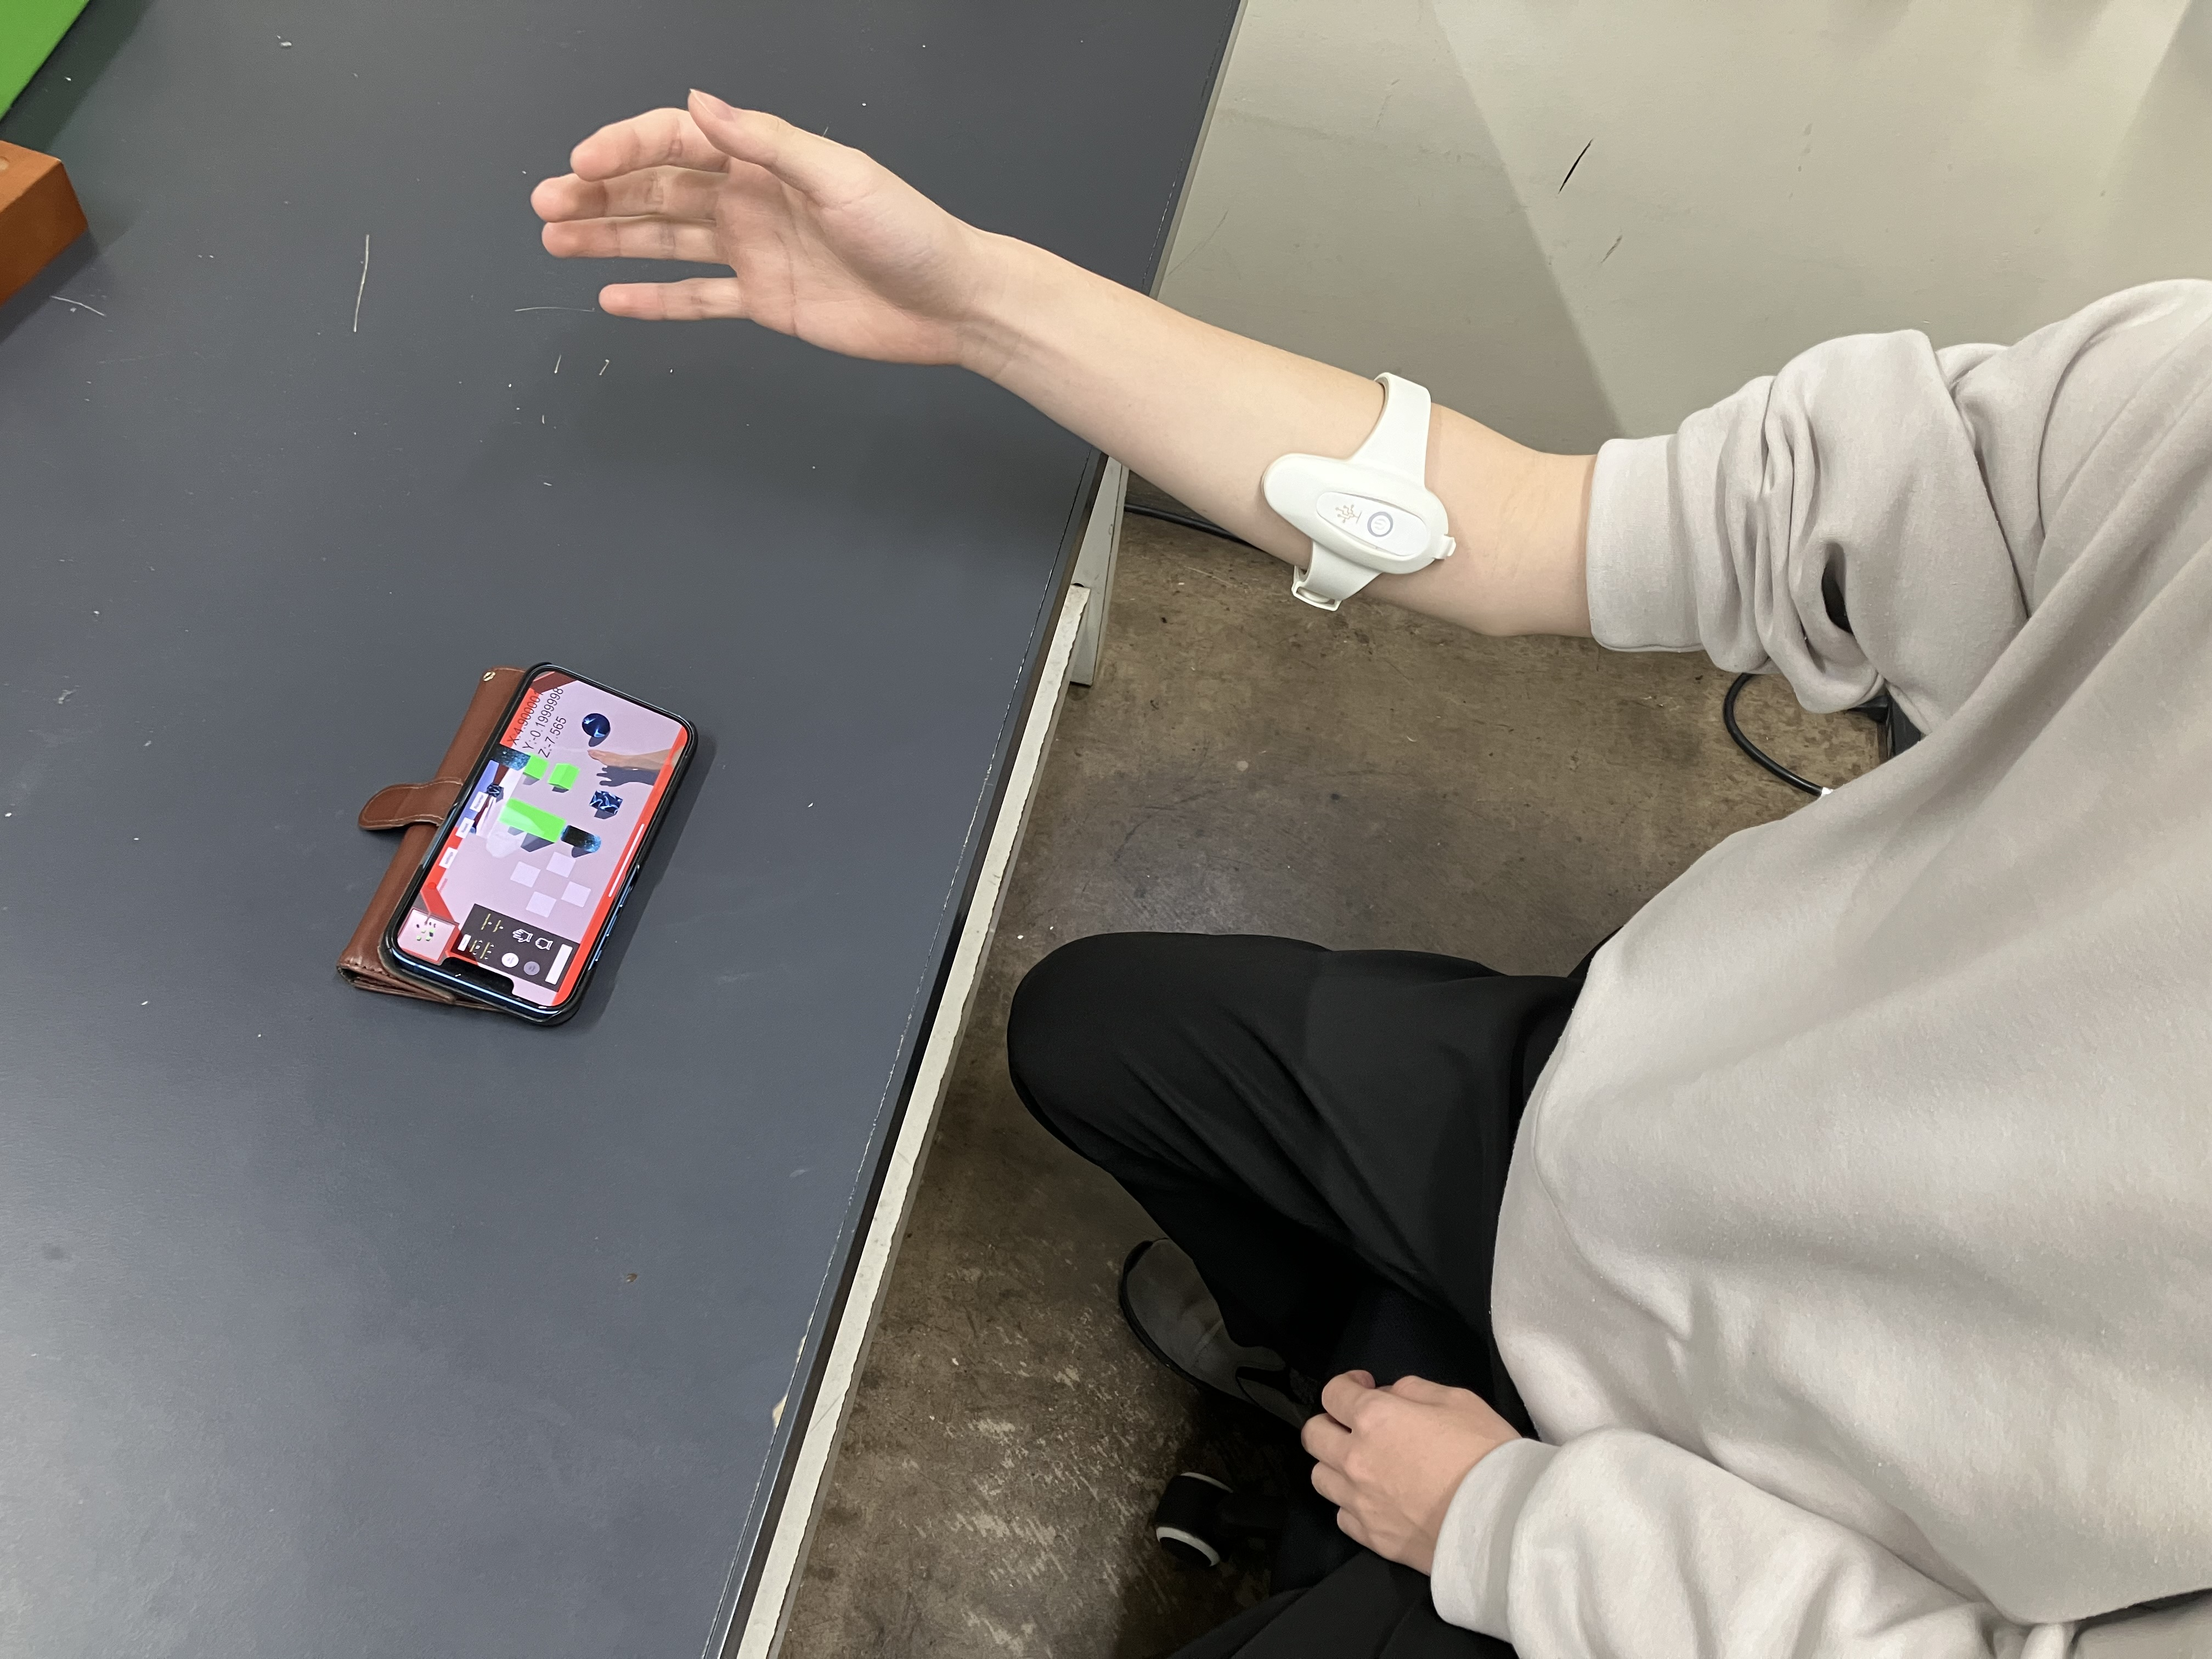
\includegraphics[width = \columnwidth]{../figs/IMG_6323.jpg}
		\end{minipage}
		\caption{シミュレータ定性評価の様子}
		\end{figure}

		\begin{figure}[H]
		\centering
		\begin{minipage}{0.45\columnwidth}
		\centering
		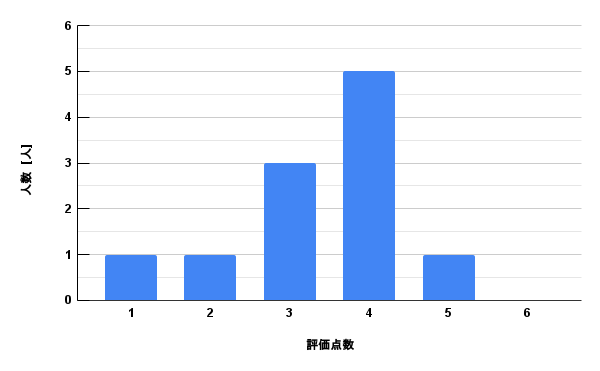
\includegraphics[width = \columnwidth]{../figs/PC-1.png}
		\end{minipage}
		\hspace{0.04\columnwidth}
		\begin{minipage}{0.45\columnwidth}
		\centering
		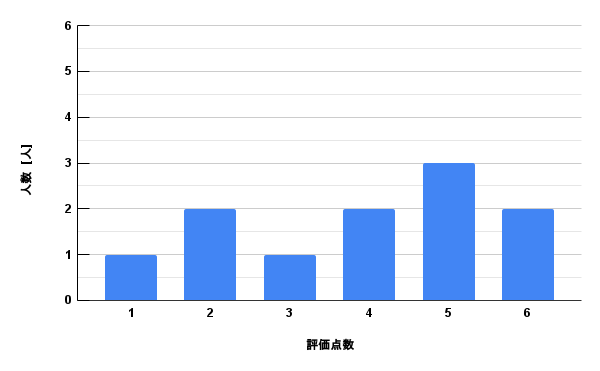
\includegraphics[width = \columnwidth]{../figs/iOS-1.png}
		\end{minipage}
		\caption{没入感の評価比較}
		\end{figure}
		PC版の平均値 3.36点 中央値は4点
		iOS版の平均値 3.90点 中央値は4点

		\begin{figure}[H]
		\centering
		\begin{minipage}{0.45\columnwidth}
		\centering
		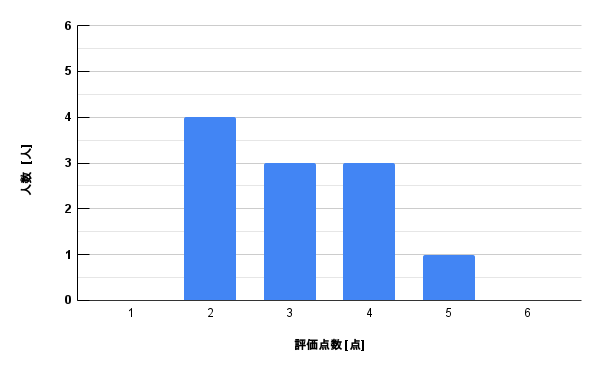
\includegraphics[width = \columnwidth]{../figs/PC-2.png}
		\end{minipage}
		\hspace{0.04\columnwidth}
		\begin{minipage}{0.45\columnwidth}
		\centering
		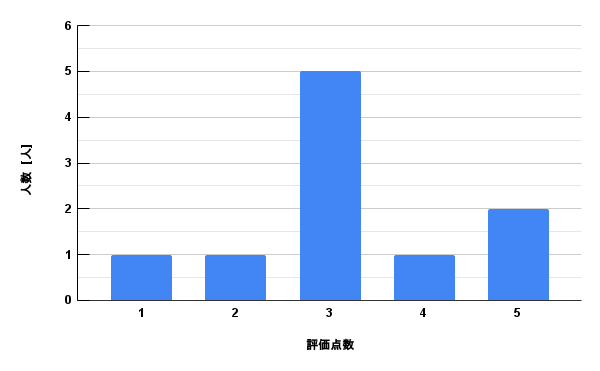
\includegraphics[width = \columnwidth]{../figs/iOS-2.png}
		\end{minipage}
		\caption{操作性の評価比較}
		\end{figure}
		PC版の平均値 3.09点 中央値 3点
		iOS版 平均値 

		\begin{figure}[H]
		\centering
		\begin{minipage}{0.45\columnwidth}
		\centering
		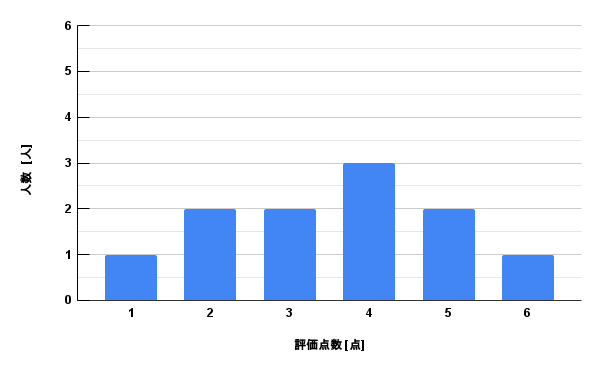
\includegraphics[width = \columnwidth]{../figs/PC-3.png}
		\end{minipage}
		\hspace{0.04\columnwidth}
		\begin{minipage}{0.45\columnwidth}
		\centering
		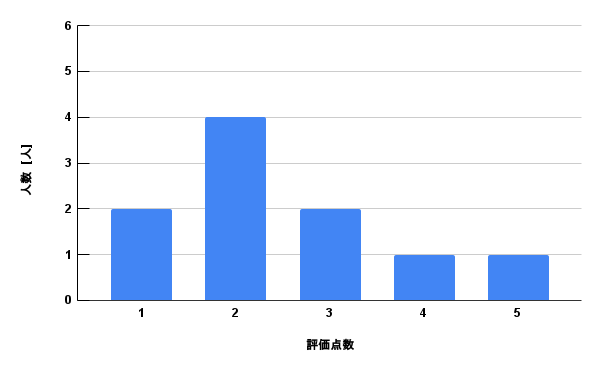
\includegraphics[width = \columnwidth]{../figs/iOS-3.png}
		\end{minipage}
		\caption{操作遅延の評価比較}
		\end{figure}

		\begin{figure}[H]
		\centering
		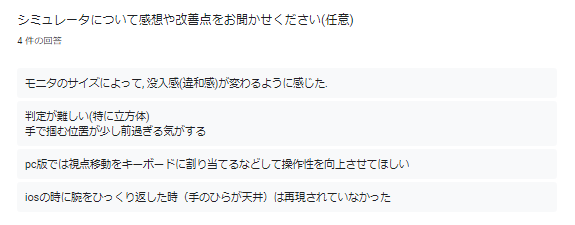
\includegraphics[width = 12cm]{../figs/result.png}
		\caption{シミュレータ定性評価のコメント}
		\label{fig:comment}
		\end{figure}

\chapter{考察}
	FirstVRを入力インターフェースとすることで実際の筋電義手を用いるより安価で
	ジェスチャ認識によってある程度オブジェクトを持ち上げと保持ができるシミュレ
	ータを構成することができた.しかし,グーのジェスチャのまま腕を動かすとジェスチャ
	状態から外れてしまうことがある.これはFirstVRが筋肉の変位を測定しているため,
	腕のひねりや向きによって筋収縮が起こり,ジェスチャのしきい値を下回ってしまう
	ためであると考えられる.また,ジェスチャに似ている動作や部分的に同じ動きをしても
	ジェスチャ状態であると判定されてしまうこともある.例えば,グーのジェスチャを
	登録した際に,手首を掌屈させるとジェスチャ状態と誤検知されてしまったり,
	じゃんけんのチョキのジェスチャをしても誤検知されてしまうこともある.
	このように,FirstVRは筋変位を測定しているため,類似する筋肉の動きで誤検知する
	場合が多いので,似たようなジェスチャを複数登録することはかなり難しい.
	だが,ジェスチャ状態が外れる腕の位置で学習回数を重ねることで少しだけ
	ジェスチャ状態が外れにくくなることがわかっている.
	この条件を調べていくことでさらに複雑なジェスチャや指の動きをトラッキング
	できるような可能性もあると考えている.

	次に,FirstVRを上肢切断者に装着してシミュレータを使ってもらうことが
	本研究の最終目的として捉えているがそもそもFirstVRで筋変位を読み取れるか
	どうか不明なことも課題点として挙げられる.後天的に切断した場合はそれまで
	にグーのジェスチャを行った経験があるため,筋肉の動きを再現することが可能
	かもしれないが,先天的に切断している場合はまずグーのジェスチャがどういう
	筋肉の状態なのかということから訓練する必要がある.
	\cite{ref:8}によると,上肢切断にはレベルが存在し,今回の実験で装着した位置はおよそ
	前腕切断に相当する位置で,本シミュレータでFirstVRを用いることができるのは
	手関節離断,前腕切断の2つである.FirstVRを上腕で用いることができるようになれば
	肘関節切断や上腕切断の状態でもシミュレータが用いることができるようなる.
	


	

	FirstVRを用いたシミュレータは\cite{ref:3}のカグラのようにVRゴーグルを用いて
	扱うことができればより訓練効果に影響があるのではないかと考えられる.
	その際はiOS版に搭載しているコントローラボタンではなくiPhoneとFirstVRの距離や
	iPhone自体のセンサを
	
	本研究では腕の3DモデルをEinScanHXによって作製したが,今後3Dスキャナが一般的に
	普及して,体格が近い人の腕をスキャンできるようになると想定すると,そのデータを
	シミュレータに用いるためにスムージングからボーン配置までを自動的に行えるアプリケーション
	があればBlenderを用いて作業する工程を省略することができるようになる.
	


\chapter{おわりに}
	本研究ではPC版のシミュレータとiOS版のシミュレータの2種類を作製し,健常者に
	体験してもらい,その定性評価を行うことでFirstVRを用いたシミュレータの方が没入感
	が高い傾向があることを示した.しかし,操作性の点ではキーボード・マウスと明確な
	差は見受けられず,遅延に関してはPC版の方が少ないという課題点も見つかった.
	また,表示するモニターの違いで没入感が違ったという意見も挙げられており,
	実験方法を再検討する必要がある.

	今後の課題としては,FirstVRの性能評価が不十分であったため,シミュレータのオブジェクト保持
	状態がノイズで保持されていない場合が多く,操作性の評価が低くなってしまったと考えられる.
	そのため,FirstVRの条件を以下に挙げる.
	\begin{itemize}
		\item 装着位置
		\item 使用者の筋肉量
		\item 学習時間
		\item 学習回数
	\end{itemize}
	これらの観点から条件を分けて実験を行う必要がある.
	また,FirstVRの内部回路の学習システムについての理解が不足しているため
	どのような条件が最適なのかということについては公式HPのリファレンスを詳しく調べていく必要が
	あると考えられる.加えて,FirstVRがスマートフォンデバイスでしか使用できない点についても
	BLE通信のスクリプトファイルを解読することでPCとの通信ができる可能性もある.
	そして,当初の目標であったオブジェクトの違いによる訓練効果の評価については
	作成したシミュレータのオブジェクトの機能を引き継いだままモデルだけ置き換えて
	シミュレータを実装することで定性評価を行うことは可能であると考える.
	定量的なデータを取得するためには脳波測定を用いての測定やシミュレータと現実空間の
	移動量の誤差などを検討していくことになるだろう.
	最後に,シミュレータの没入感をあげる方法として,VRゴーグルを用いたシステムにできると
	より訓練効果などに影響を与えられるのではないかと思われる.
\clearpage

\chapter*{謝辞}
\addcontentsline{toc}{chapter}{謝辞}
一年間丁寧に指導していただいた戸崎 哲也教授,および同研究室の村岡 永遠君に深く感謝いたします.
また,実験に協力いただいた電子工学科の31名にも深く感謝いたします.

\begin{thebibliography}{99}

	\bibitem{ref:1}
	芝軒 太郎 他.``VRを利用した筋電義手操作トレーニング
	システムの開発と仮想 Box and Block Test の実現''.
	JRSJ. 2012 July.

	\bibitem{ref:2}
	Osumi M, et.al.
	``Characteristics of Phantom Limb Pain Alleviated
	with Virtual Reality Rehabilitation''.
	Pain Med. 2019 May.

	\bibitem{ref:3}
	mediVR.Inc.,https://www.medivr.jp/
	最終閲覧日 2023/01/31


	\bibitem{ref:4}
	株式会社サンステラ, https://www.einscan.jp/einscan-hx
	
	
	
	\bibitem{ref:5}
	H2L.Inc.,Tokyo106-0032,Japan;satoshi.hosono@h2l.jp
	


	\bibitem{ref:6}
	Tamon Miyake, et.al.``Gait Phase Detection Based on Muscle Deformation
	with Static Standing-Based Calibration''.
	MDPI. 2021 Feb pp.05,13.


	\bibitem{ref:7}
	JEOL,``平滑化(スムージング)''\\
	https://www.jeol.co.jp/words/emterms/20121023.094657.html\#gsc.tab=0
	最終閲覧日 2023/01/31

	\bibitem{ref:8}
	ottobock,``上肢の切断レベル''\\
	https://www.ottobock.com/ja-jp/prosthetic\_ue/info/amputation\_level
	最終閲覧日 2023/02/01

\end{thebibliography}

\chapter*{付録}

%目次に付録を追加
\addcontentsline{toc}{chapter}{付録}
%ページ番号をローマ数字で表示
\pagenumbering{roman}


\appendix
%章番号をアルファベットに変換
\renewcommand{\thesection}{\Alph{chapter}.\arabic{section}}
\setcounter{chapter}{1}

\section{測定データ}
	FirstVRの性能評価の際に取得したデータを図\refeq{fig:QRcode}に示す.
	\begin{figure}[H]
	\centering
	
\includegraphics[width = 6cm]{../figs/QRshare.png}
	\caption{FVRDataFilesのQRコード}
	\label{fig:QRcode}
	\end{figure}
	
\section{ソースコード}
\begin{lstlisting}[caption = CalibrationManager, label = code:Calibration]
using System.Collections;
using System.Collections.Generic;
using UnityEngine;
using UnityEngine.XR;
using UnityEngine.UI;
using UnityEngine.Animations;
using System.Linq;
using FVRlib;
public class CalibrationManager : MonoBehaviour
{
    public Animator animator;
    public GameObject Collider;
 
    public Transform GrapPoint_sphere, GrapPoint_cylinder, GrapPoint_cube;

    // FVR 
    public FVRConnection fvr;
    public FVRGesture gesture;

    //Control variables
    int samplesPerSecond = 0;
    int roundLength = 0;
    int tCalibRounds = 0;
    int ntCalibRounds = 0;

    // Texts
    public Text samplesPerSecondTxt;
    public Text roundLengthTxt;
    public Text tCalibRoundsTxt;
    public Text ntCalibRoundsTxt;

    // Images
    public Image targetImg;
    public Image nonTargetImg;
    public Image testImg;

    //Buttons
    public Button targetBtn;
    public Button nonTargetBtn;
    public Button resetBtn;
    public Button[] varBtns;

    bool cube_col;
    bool cylinder_col;
    bool sphere_col;

    // int grap;

    // Start is called before the first frame update
    void Start()
    {
        fvr = FindObjectOfType (typeof(FVRConnection)) as FVRConnection;

        // Create a new custom gesture
        gesture = fvr.gestureManager.RegisterCustomGesture ("gestureName");

        // Display the default settings
        samplesPerSecond = fvr.gestureManager.calibrationSamplesPerSecond;
        roundLength = (int)fvr.gestureManager.calibrationRoundLength;
        UpdateTexts ();

        // Button control
        targetBtn.interactable = false;
    }

    void Update()
    {
        Vector3 origin = Collider.transform.position;
        Vector3 direction = -Collider.transform.forward;
        Ray ray = new Ray(origin,direction);
        Debug.DrawRay(ray.origin, ray.direction*0.2f, Color.red, 0.01f);
        if(Physics.Raycast(ray, out RaycastHit hit, 1.0f))
        {
            Debug.Log(hit.collider.gameObject.name);
            if(hit.collider.gameObject.name == "Cube")
                cube_col = true;
            if(hit.collider.gameObject.name == "Cylinder")
                cylinder_col  = true;
            if(hit.collider.gameObject.name == "Sphere")
                sphere_col = true;
        }

        if(gesture.held == true)
        {
            animator.SetBool("grap_null",true);
            testImg.color = Color.green;
            if(cube_col == true)
            {
                testImg.color = Color.blue;
                animator.SetBool("grap_cube1",true);
				GameObject cube = GameObject.Find("Cube");
				Rigidbody rb = cube.GetComponent<Rigidbody>();
				rb.isKinematic = true;
				cube.transform.position = GrapPoint_cube.position;
				cube.gameObject.transform.parent = GrapPoint_cube;
            }
            if(cylinder_col == true)
            {
                testImg.color = Color.red;
                animator.SetBool("grap_cylinder1",true);
				GameObject cylinder = GameObject.Find("Cylinder");
				Rigidbody rb = cylinder.GetComponent<Rigidbody>();
				rb.isKinematic = true;
				cylinder.transform.position = GrapPoint_cylinder.position;
				cylinder.gameObject.transform.parent = GrapPoint_cylinder;
            }
            if(sphere_col == true)
            {
                testImg.color = Color.yellow;
                animator.SetBool("grap_sphere1",true);
				GameObject sphere = GameObject.Find("Sphere");
				Rigidbody rb = sphere.GetComponent<Rigidbody>();
				rb.isKinematic = true;
				sphere.transform.position = GrapPoint_sphere.position;
				sphere.gameObject.transform.parent = GrapPoint_sphere;
            }
        }
        else if(gesture.held == false)
        {
            testImg.color = Color.white;

            animator.SetBool("grap_null",false);
            animator.SetBool("grap_sphere1", false);
            animator.SetBool("grap_cylinder1", false);
            animator.SetBool("grap_cube1", false);

            cube_col = false;
            cylinder_col = false;
            sphere_col = false;

            //sphere
            GameObject sphere = GameObject.Find("Sphere");
            Rigidbody rb_sphere = sphere.GetComponent<Rigidbody>();
            rb_sphere.isKinematic = false;
            sphere.gameObject.transform.parent = null;

            //cylinder
            GameObject cylinder = GameObject.Find("Cylinder");
            Rigidbody rb_cylinder = cylinder.GetComponent<Rigidbody>();
            rb_cylinder.isKinematic = false;
            cylinder.gameObject.transform.parent = null;

            //cube
            GameObject cube = GameObject.Find("Cube");
            Rigidbody rb_cube = cube.GetComponent<Rigidbody>();
            rb_cube.isKinematic = false;
            cube.gameObject.transform.parent = null;
        }
    }

    public void ChangeSPS(int dir){
        samplesPerSecond += 1 * dir;
        samplesPerSecond = samplesPerSecond < 1 ? 1 : samplesPerSecond;
        fvr.gestureManager.calibrationSamplesPerSecond = samplesPerSecond;
        UpdateTexts ();
    }
	/// <summary>
	/// You can change the length of the calibration round.
	/// This length should always be higher than 0 and making it too long might affect the results in a negative way.
	/// Recomended values are 1~3
	/// </summary>
    public void ChangeRL(int dir){
        roundLength += 1 * dir;
        roundLength = roundLength < 1 ? 1 : roundLength;
        fvr.gestureManager.calibrationRoundLength = (float)roundLength;
        UpdateTexts ();
    }

    public void SetTargetPress(){
        StartCoroutine (Calibrate (true));
    }

    public void SetNonTargetPress(){
        StartCoroutine (Calibrate (false));
    }

    // Reset the calibration data and start all over again
    public void ResetCalibrationPress(){
        fvr.gestureManager.ResetPatternData (gesture);
        tCalibRounds = 0;
        ntCalibRounds = 0;
        UpdateTexts ();
        targetBtn.interactable = false;
        nonTargetBtn.GetComponentInChildren<Text> ().text = "Set\nDummy";
        foreach (Button b in varBtns) {
            b.interactable = true;
        }
    }

    // Updates the display texts
    void UpdateTexts(){
        tCalibRoundsTxt.text = tCalibRounds.ToString ();
        ntCalibRoundsTxt.text = ntCalibRounds.ToString ();
        samplesPerSecondTxt.text = samplesPerSecond.ToString ();
        roundLengthTxt.text = roundLength.ToString ();
    }

    /// <summary>
    /// Calibrate the gesture with target or non-target values.
    /// Calibration requires time, and it's best to let the user know what's going on, so this process is best done in a coroutine.
    /// </summary>
    IEnumerator Calibrate(bool target){
        if (target) {
            // Setting target values
            fvr.gestureManager.SetTargetData (gesture);
            tCalibRounds++;
        } else {
            // Setting non-target values
            fvr.gestureManager.SetNonTargetData (gesture);
            /// The first time we set a target or non-target value, the round length and samples per second are ignored and the SVM takes only one value with dummy data then
            /// the dummy data is replaced with real data. 
            /// After the first round the FVRGesture.calibrated flag is set to true and you are ready to start calibrating with real data
            if (gesture.calibrated) {
                ntCalibRounds++;
            }else{
                nonTargetBtn.GetComponentInChildren<Text> ().text = "Set\nNonTarget";
                foreach (Button b in varBtns) {
                    b.interactable = false;
                }
            }
        }
        // We dont wan't multiple coroutines taking the same data so it's good to block the user from starting a new one before this round is done
        targetBtn.interactable = false;
        nonTargetBtn.interactable = false;
        resetBtn.interactable = false;
        float t = 0;
        while (gesture.registering) {
            /// While the target or non-target data is being set, the FVRGesture.registering flag will be set to true.
            /// A count down or a image fill loading bar is a good way to let the user know your app is doing something.
            /// Once the porcess is done, the FVRGesture.registering flag will be set to false, and we will exit this while loop.
            t += Time.deltaTime;
            if(target)
                targetImg.fillAmount = t / (float)roundLength;
            else
                nonTargetImg.fillAmount = t / (float)roundLength;
            yield return null;
        }
        UpdateTexts ();
        targetImg.fillAmount = 0;
        nonTargetImg.fillAmount =0;
        // After the process is done you can enable whatever buttons you need to proceed with the calibration or move on with your app.
        targetBtn.interactable = true;
        nonTargetBtn.interactable = true;
        resetBtn.interactable = true;
    }
}

\end{lstlisting}

\clearpage

\begin{lstlisting}[caption=MoveManager.cs, label=code:Move]
	using System.Collections;
using System.Collections.Generic;
using UnityEngine;

public class Movemanager : MonoBehaviour
	{
		public Vector3 Up_speed,Down_speed,Left_speed,Right_speed;
		bool forwardmove;
		bool backmove;
		bool rightmove;
		bool leftmove;

		public void forwardButtonDown(){
			forwardmove = true;
		}
		public void forwardButtonUp(){
			forwardmove = false;
		}
		public void backButtonDown(){
			backmove = true;
		}
		public void backButtonUp(){
			backmove = false;
		}
		public void rightButtonDown(){
			rightmove = true;
		}
		public void rightButtonUp(){
			rightmove = false;
		}
		public void leftButtonDown(){
			leftmove = true;
		}
		public void leftButtonUp(){
			leftmove = false;
		}
		void Update()
		{
			if(forwardmove == true){
				transform.position += Up_speed;
			}
			if(backmove == true){
				transform.position += Down_speed;
			}
			if(rightmove == true){
				transform.position += Right_speed;
			}
			if(leftmove == true){
				transform.position += Left_speed;
			}
		}
	}
\end{lstlisting}

\begin{lstlisting}[caption=handtrack.cs, label=code:track]
	using System.Collections;
	using System.Collections.Generic;
	using UnityEngine;
	using FVRlib;

	public class handtrack : MonoBehaviour
	{
		public FVRConnection fvr;

		// Update is called once per frame
		void Update()
		{
			this.transform.rotation = fvr.centeredRotation;
		}
	}
\end{lstlisting}

\end{document}